\section{像差类型分析与像质评估}

\subsection{单色像差与矫正方法}

\englishtitle{Characteristics of Spherical Aberration}
\begin{frame}{球差的特征}
    \begin{columns}[T]
        \begin{column}{.45\textwidth}
            \begin{figure}
                \centering
                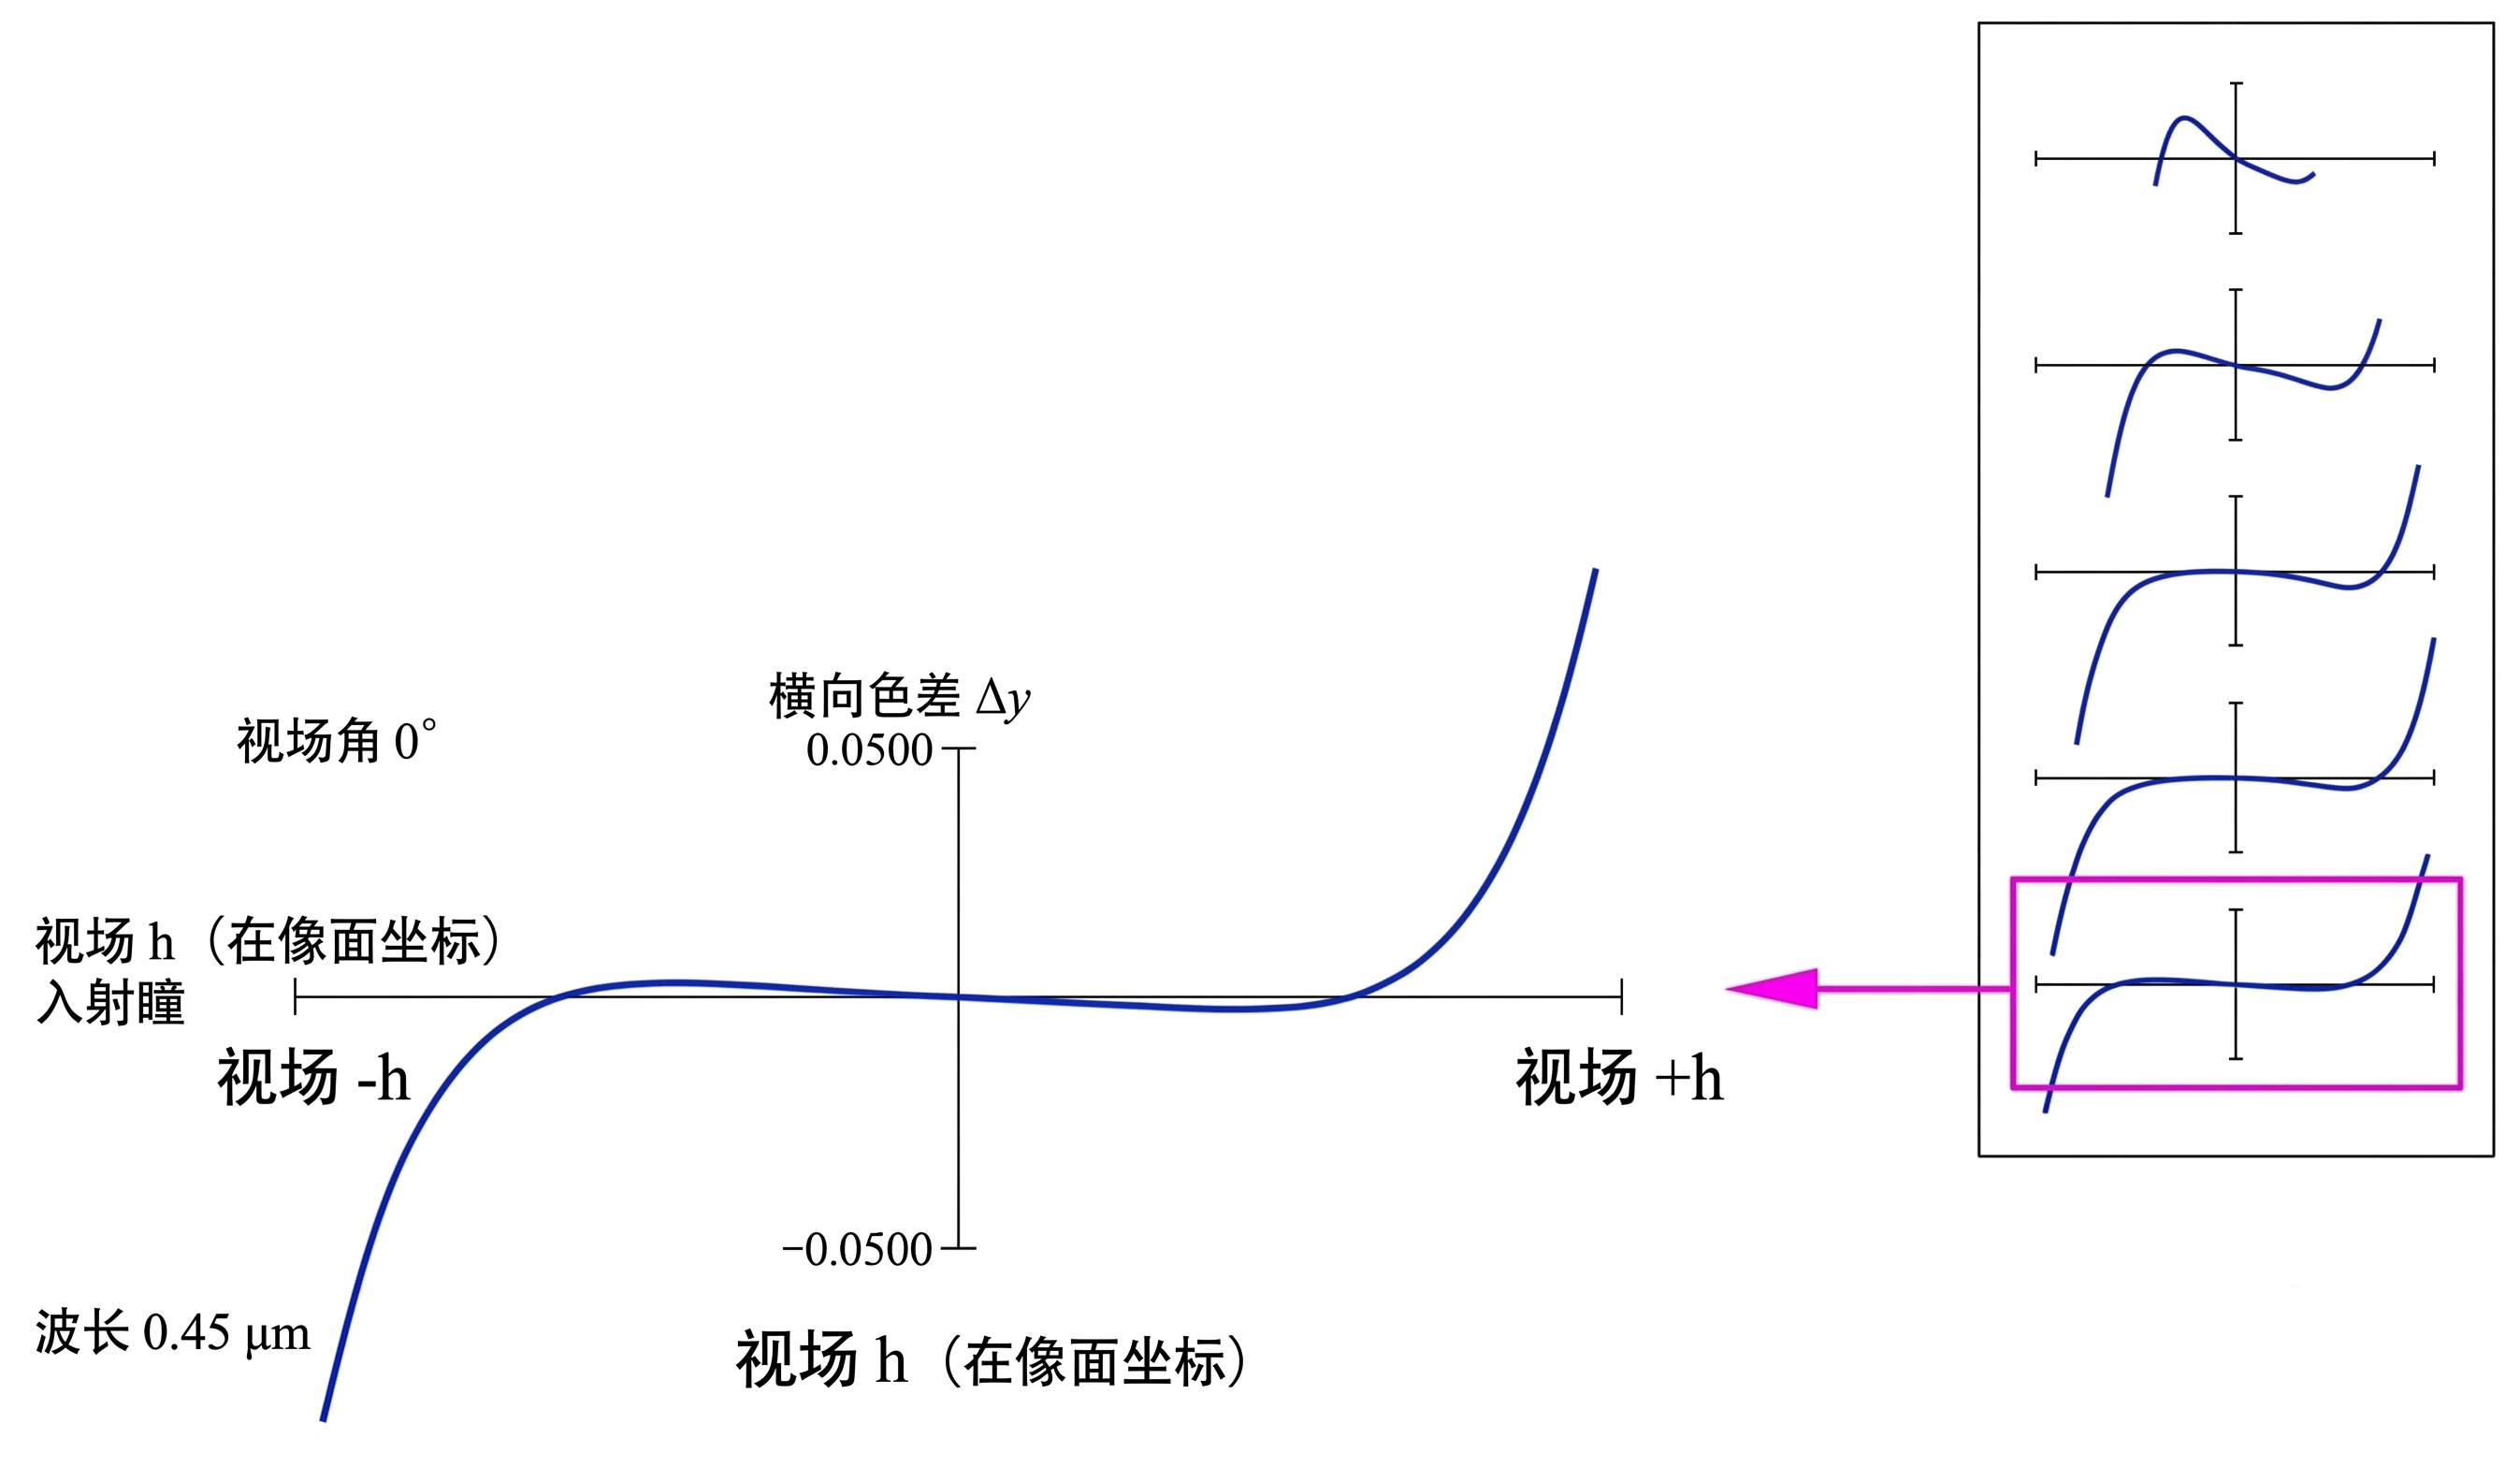
\includegraphics[width=0.95\textwidth]{Figure/图片23.png}
                \caption{球差引起的横向像差图——三次曲线}
                \label{fig:spherical}
            \end{figure}
        \end{column}
        \hfill
        \begin{column}{.55\textwidth}
            \textbf{球差(Spherical Aberration)：}
            \bigbreak
            轴上光束中出现的\alert{唯一单色像差}。与孔径三次方成正比，横向像差图表现为\alert{三次曲线}(奇函数)。可包含3阶、5阶、7阶等奇函数分量。

            \bigbreak
            \textbf{混合像差：}实际系统中球差很少单独出现，通常与离焦分量和高阶球差混合。

            \bigbreak
            \alert{需要将各成分分解分析，才能有效优化镜头性能。}
        \end{column}
    \end{columns}
\end{frame}

\englishtitle{Correction Methods for Spherical Aberration}
\begin{frame}{球差矫正方法}
    \begin{block}{球差的定义}
        轴上光线与边缘光线在光轴上焦点之间的\alert{轴向距离}即为球差。
    \end{block}

    \textbf{主要矫正策略：}
    \begin{enumerate}
        \item \alert{分摊光焦度}：将单个透镜的光焦度分配给多个透镜，减小每个面的曲率
        \item \alert{透镜拆分}：用大曲率半径的多个透镜替代小曲率半径的单一透镜
        \item \alert{胶合透镜}：利用正负透镜的球差符号相反进行相互抵消
        \item \alert{非球面透镜}：通过改变面形消除球差(最理想方式)
    \end{enumerate}

    \alert{核心思路：}球差源于球面折射面的几何形状，通过改变面形或光焦度分配来减小不同孔径区域的折射角度差异。
\end{frame}

\englishtitle{Characteristics and Types of Coma}
\begin{frame}{彗差的特征与类型}
    \begin{columns}[T,onlytextwidth]
        \begin{column}{.55\textwidth}
            \begin{block}{\footnotesize 光路图与横向像差图对比}
                \centering
                \begin{minipage}[t]{.49\linewidth}
                    \centering
                    {\scriptsize \alert{外向彗差}}
                    \par\vspace{2pt}
                    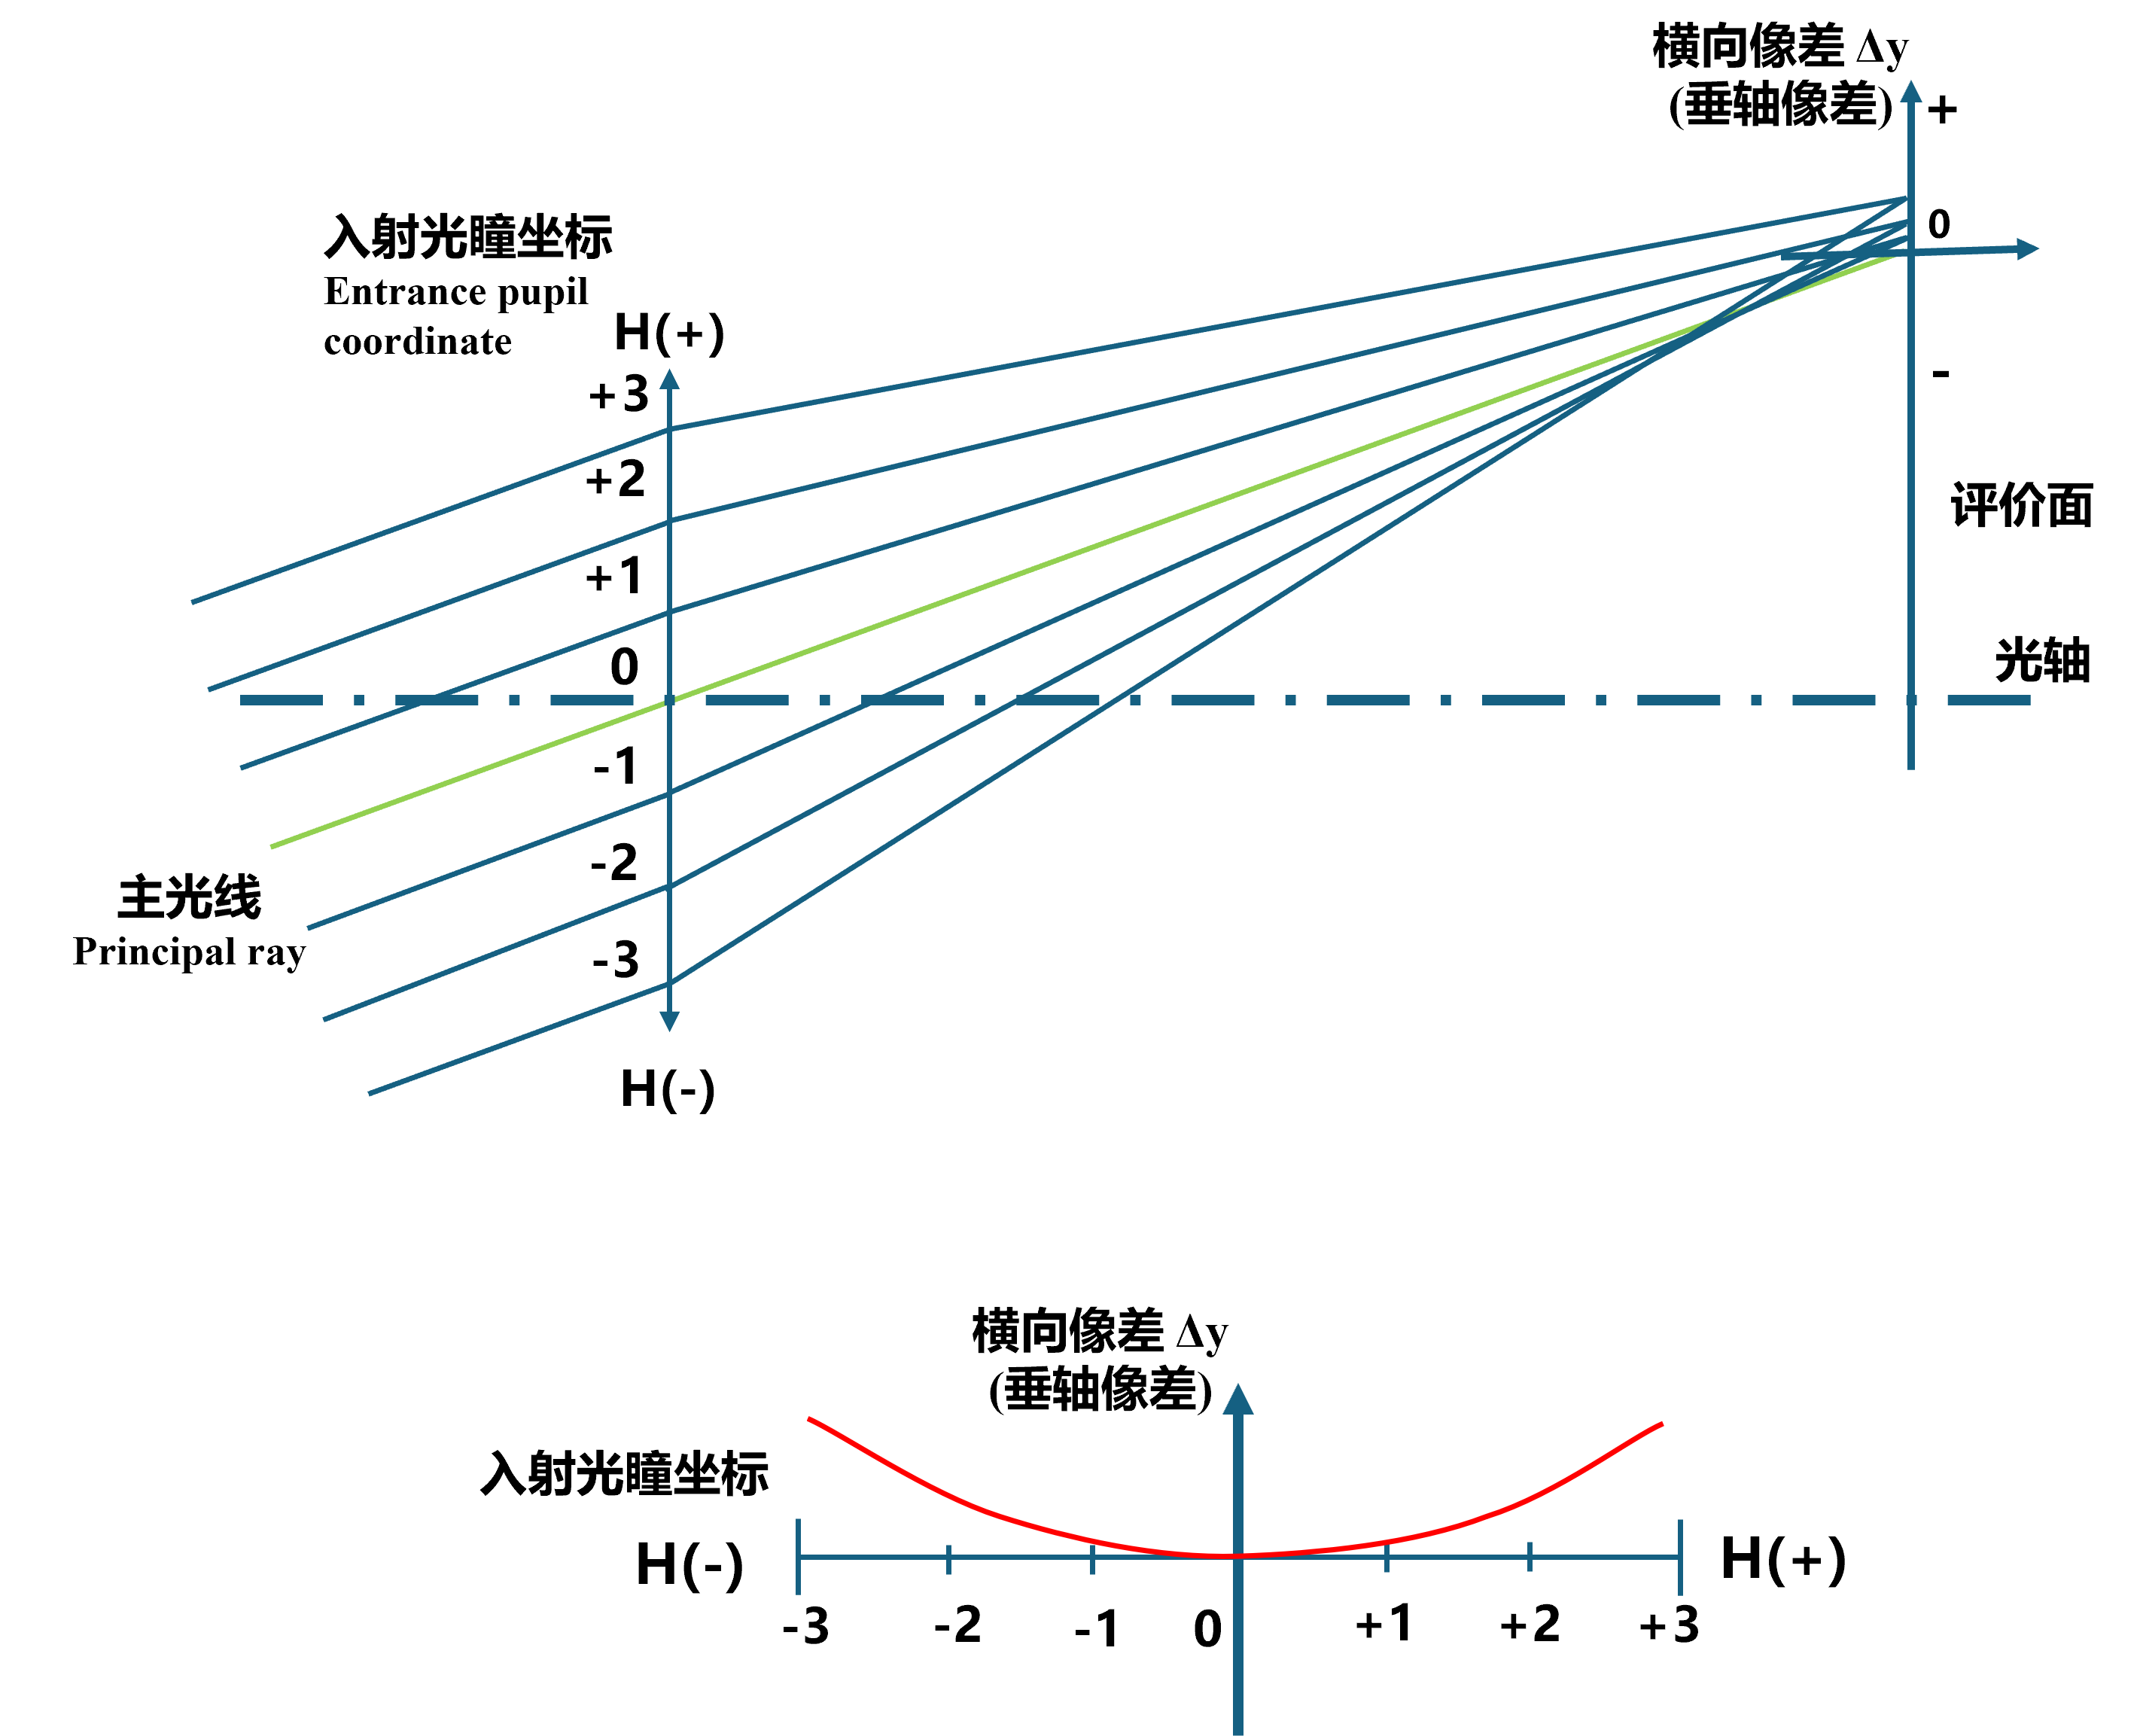
\includegraphics[width=\linewidth,height=.34\textheight,keepaspectratio]{Figure/图片8.png}
                    \par\vspace{2pt}
                    {\scriptsize 下凸二次曲线}
                    \label{fig:outward_coma}
                \end{minipage}
                \hfill
                \begin{minipage}[t]{.49\linewidth}
                    \centering
                    {\scriptsize \alert{内向彗差}}
                    \par\vspace{2pt}
                    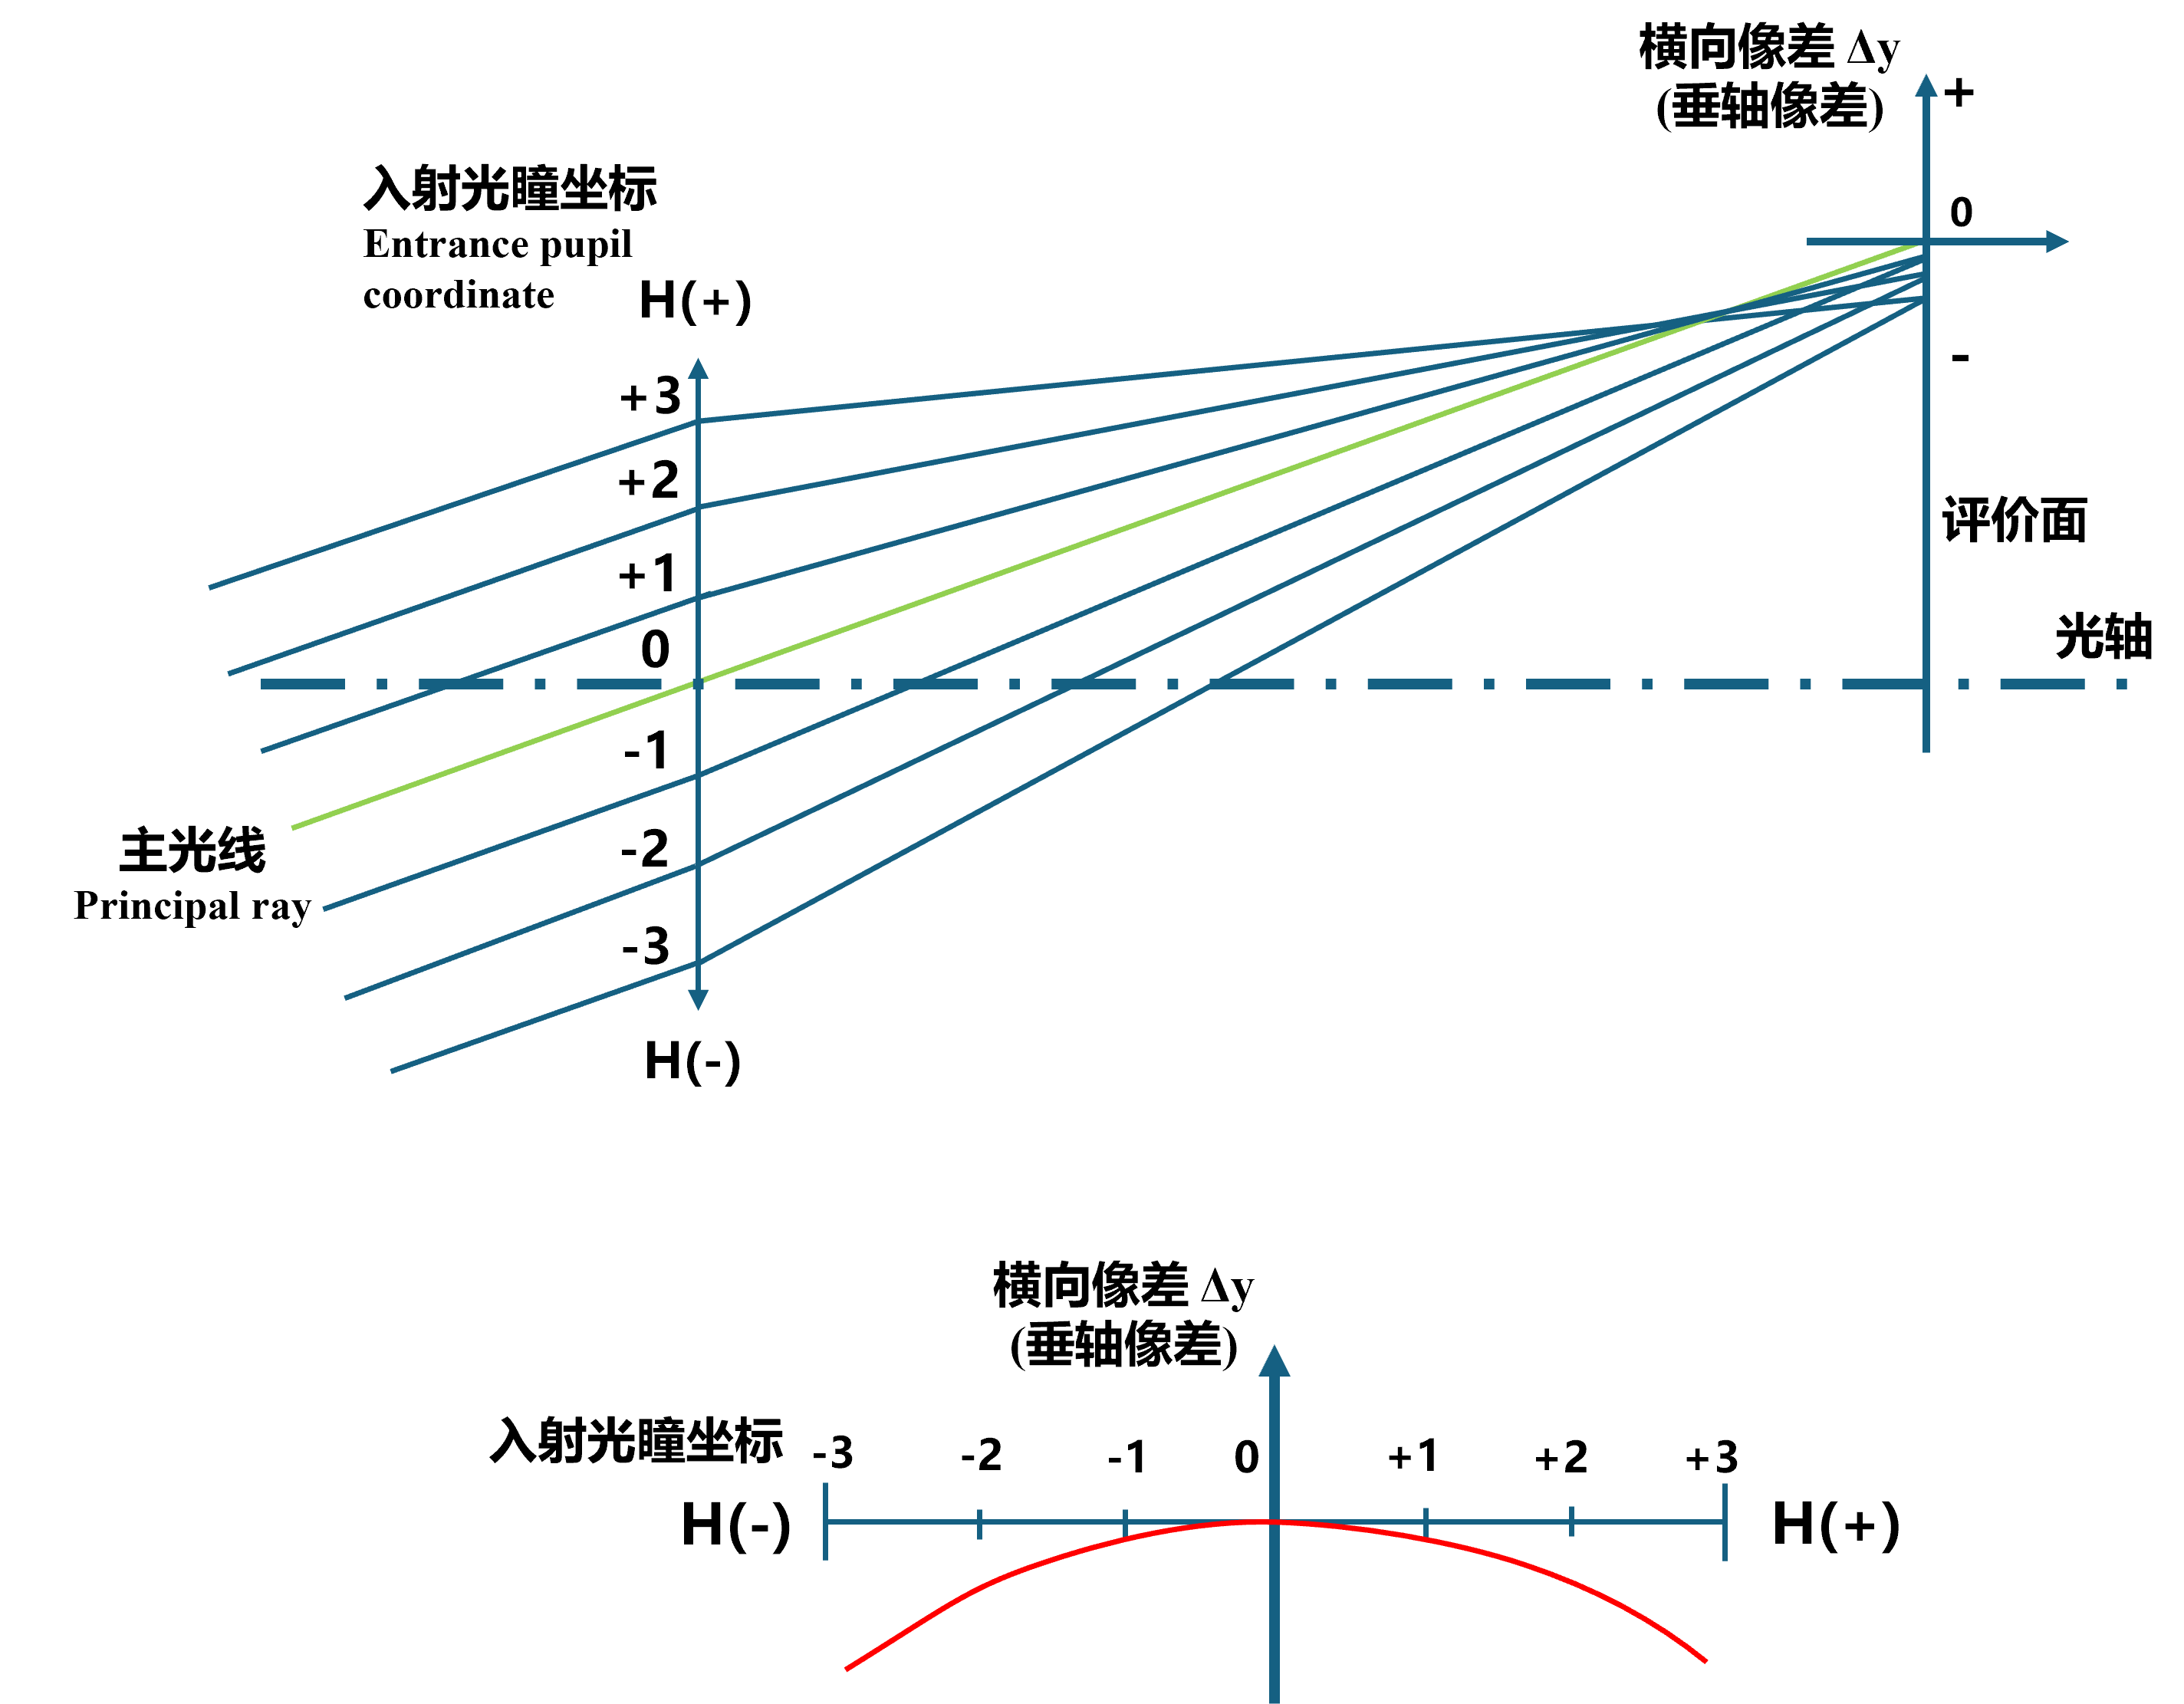
\includegraphics[width=\linewidth,height=.34\textheight,keepaspectratio]{Figure/图片11.png}
                    \par\vspace{2pt}
                    {\scriptsize 上凸二次曲线}
                    \label{fig:inward_coma}
                \end{minipage}
            \end{block}
        \end{column}
        \hfill
        \begin{column}{.43\textwidth}
            \begin{block}{\footnotesize 彗差的定义}
                \small
                横向像差图关于入射光瞳坐标呈\alert{二次函数关系}的像差。与 $h^2$ 成正比(偶函数)。
            \end{block}

            \vspace{2pt}
            \small
            \textbf{两种类型及判断：}
            \begin{enumerate}
                \setlength{\itemsep}{3pt}
                \item \alert{外向彗差}：\alert{下凸}二次曲线
                \begin{itemize}
                    \setlength{\itemsep}{-1pt}
                    \item 上侧光线穿过主光线后落在正侧
                \end{itemize}
                \item \alert{内向彗差}：\alert{上凸}二次曲线
                \begin{itemize}
                    \setlength{\itemsep}{-1pt}
                    \item 上侧光线与主光线交叉后落在负侧
                \end{itemize}
            \end{enumerate}

            \vspace{2pt}
            {\small \alert{要点：}看横向像差曲线的开口方向，而不是只看光线图的倾斜程度。}
        \end{column}
    \end{columns}
\end{frame}

\englishtitle{Coma Diagnosis and Correction}
\begin{frame}{彗差判断与矫正}
    \begin{columns}[T]
        \begin{column}{.50\textwidth}
            \textbf{如何判断彗差：}
            \begin{itemize}
                \item 横向像差图呈 $\propto h^2$ 的二次曲线
                \item 下凸 $\rightarrow$ 外向彗差 / 上凸 $\rightarrow$ 内向彗差
                \item 离焦\alert{无法改善}彗差——这是区分彗差与离焦的关键
                \item 彗差属偶函数，球差属奇函数
            \end{itemize}
        \end{column}
        \hfill
        \begin{column}{.50\textwidth}
            \textbf{彗差矫正策略：}
            \begin{enumerate}
                \item \alert{改变光阑位置}：满足阿贝正弦条件
                \item \alert{非球面透镜}：改变轴外光线折射角分布
                \item \alert{对称光学结构}：前后对称抵消奇次彗差
            \end{enumerate}

            \alert{注意：}彗差本质是\alert{轴外球差}，在\alert{大孔径+大视场}时最严重。
        \end{column}
    \end{columns}
\end{frame}

\englishtitle{Hidden Coma}
\begin{frame}{隐性彗差}
    \begin{columns}[T]
        \begin{column}{.50\textwidth}
            \begin{figure}
                \centering
                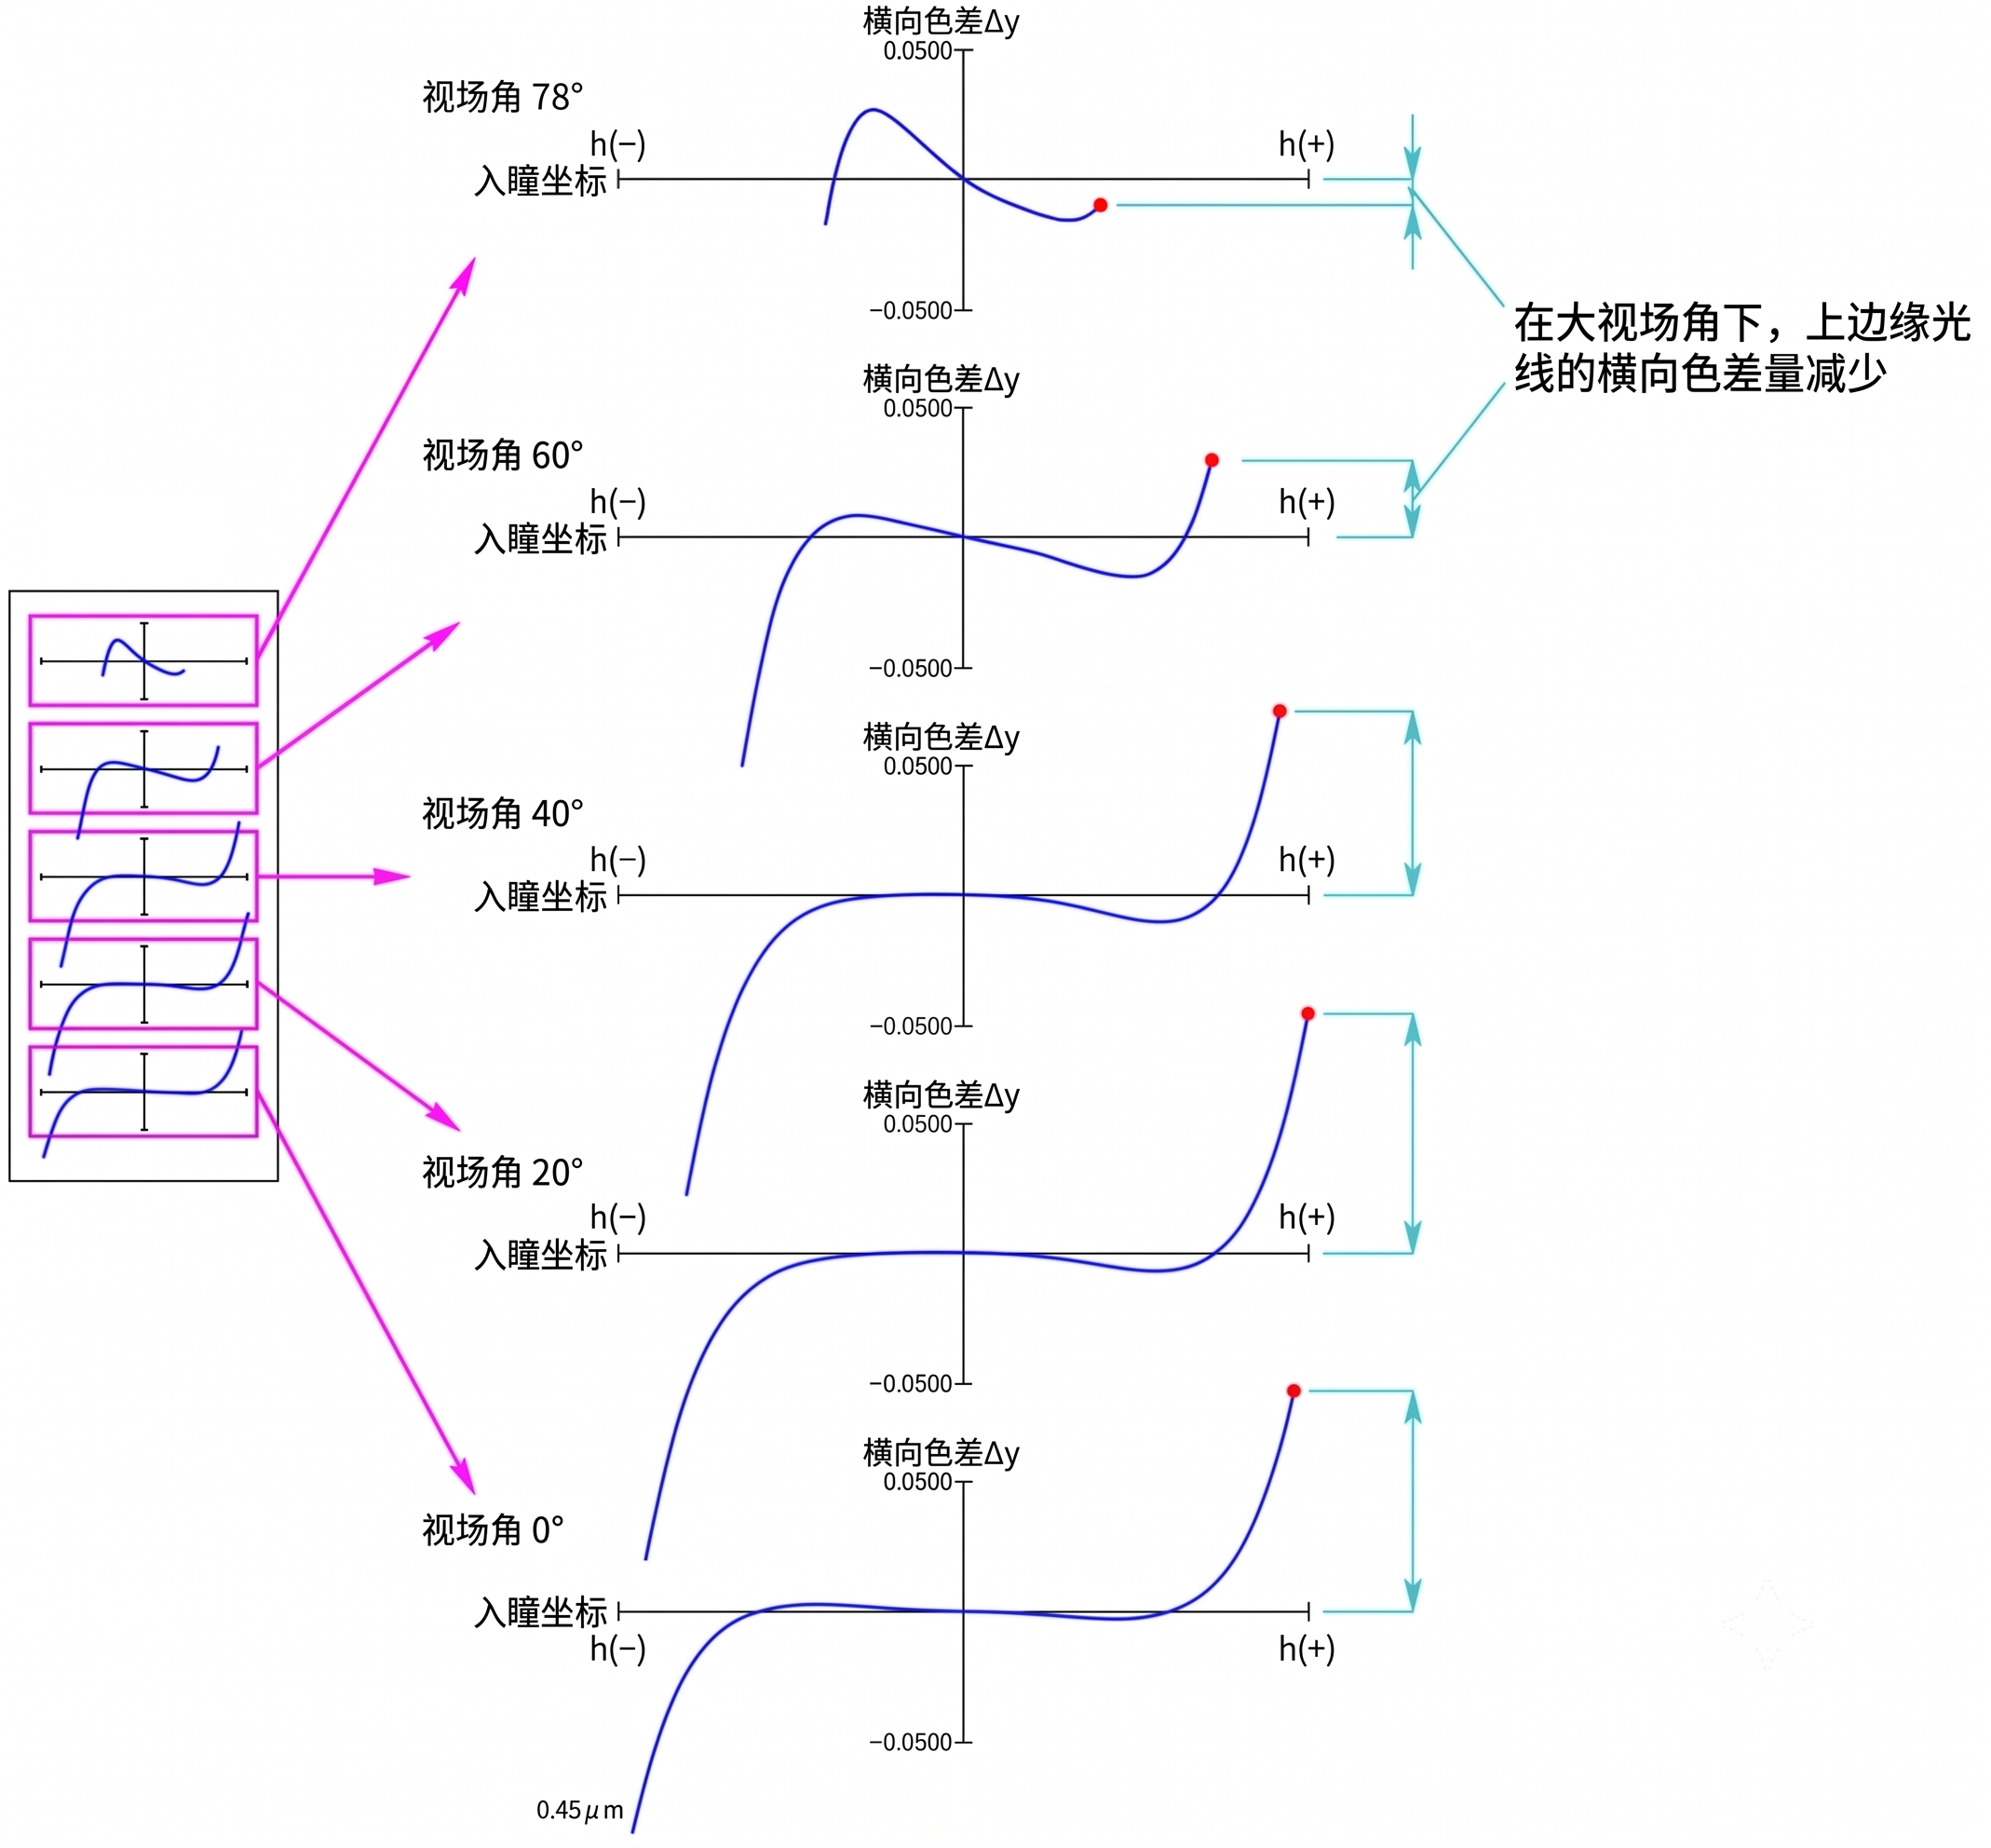
\includegraphics[width=0.9\textwidth]{Figure/图片24.png}
                \caption{隐性彗差——上边缘光线随视场增大而减小}
                \label{fig:hidden_coma}
            \end{figure}
        \end{column}
        \hfill
        \begin{column}{.50\textwidth}
            典型光学系统中，横向像差包含\alert{离焦、球差、彗差和场曲}的复合分量。

            \bigbreak
            \textbf{隐性彗差的特征：}
            \begin{itemize}
                \item 上边缘光线像差随视场增大而\alert{减小}
                \item 下边缘光线像差\alert{基本不变}
                \item 球差(奇函数)和彗差(偶函数)叠加
            \end{itemize}

            \bigbreak
            \textbf{机制：}上边缘二者\alert{抵消}，下边缘二者\alert{加强}。
        \end{column}
    \end{columns}
\end{frame}

\englishtitle{Transverse Aberration of Field Curvature}
\begin{frame}{场曲的横向像差图特征}
    \begin{columns}[T]
        \begin{column}{.35\textwidth}
            \begin{figure}
                \centering
                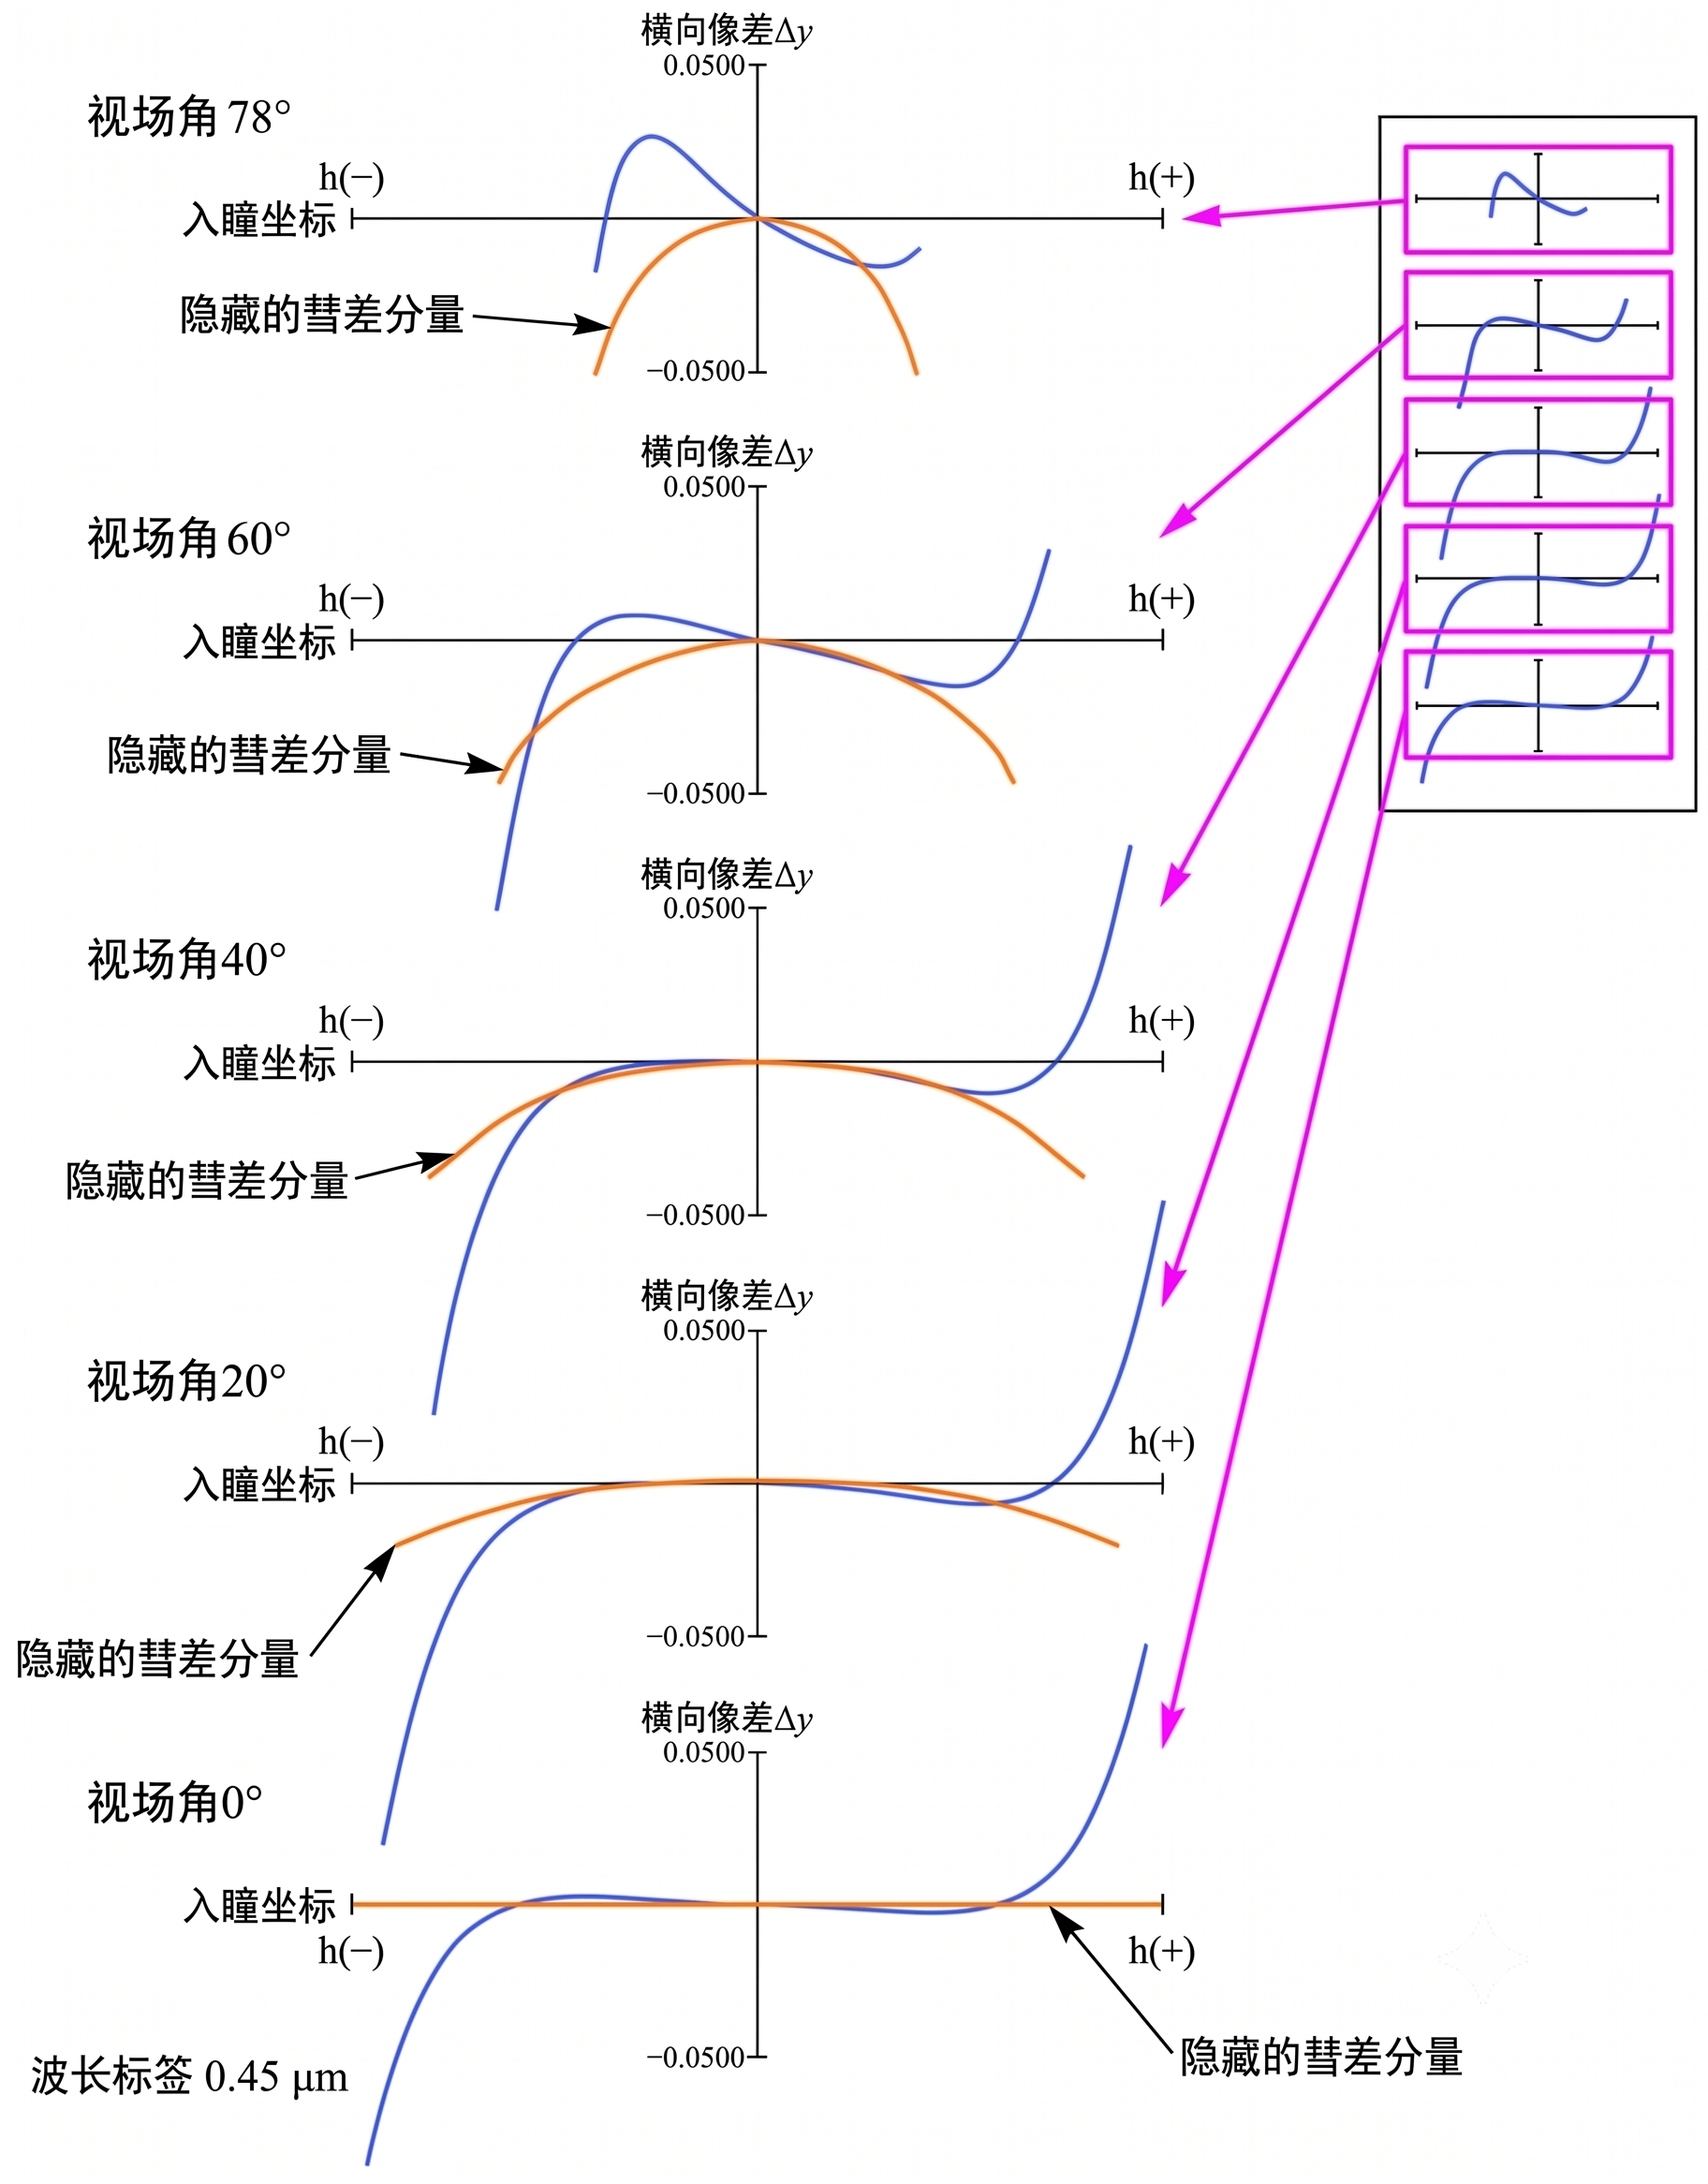
\includegraphics[width=0.9\textwidth]{Figure/图片25.png}
                \caption{场曲——原点附近斜率因视场而异}
                \label{fig:field_curvature}
            \end{figure}
        \end{column}
        \hfill
        \begin{column}{.65\textwidth}
            \textbf{场曲(Field Curvature)：}
            即使物面是平面，像面也可能弯曲——\alert{场曲}。

            \bigbreak
            \textbf{识别方法：}横向像差图\alert{原点附近}斜率因视场角不同而不同。

            \bigbreak
            各视场成像点在纵向上\alert{不同}，连接后形成\alert{弯曲的像面}(Petzval曲面)。

            \bigbreak
            \textbf{为何关注原点附近？}
            \begin{itemize}
                \item 球差($h^3$)和彗差($h^2$)在此处影响极小
                \item 场曲($h^1$)在原点附近\alert{占主导}
            \end{itemize}
        \end{column}
    \end{columns}
\end{frame}

\englishtitle{Correction Methods for Field Curvature}
\begin{frame}{场曲矫正方法}
    \begin{columns}[T]
        \begin{column}{.52\textwidth}
            \textbf{佩兹伐和(Petzval Sum)控制：}
            场曲受系统的佩兹伐和支配，核心是\alert{降低总佩兹伐和}。

            \textbf{主要策略：}
            \begin{enumerate}
                \item \alert{正负光焦度分离}：正负透镜组合抵消佩兹伐贡献
                \item \alert{弯月透镜}：特殊面形引入负佩兹伐贡献
                \item \alert{场镜}：在像面前改变会聚角而不影响总光焦度
            \end{enumerate}
        \end{column}
        \hfill
        \begin{column}{.48\textwidth}
            \begin{block}{佩兹伐条件(薄透镜)}
                \begin{equation}
                    \sum \frac{\phi_i}{n_i} \rightarrow 0
                    \label{eq:petzval}
                \end{equation}
                其中 $\phi_i$ 为光焦度，$n_i$ 为折射率。

                正负透镜组合是\alert{唯一}能同时校正场曲和维持总光焦度的手段。
            \end{block}
        \end{column}
    \end{columns}
\end{frame}

\englishtitle{Meridional Plane, Sagittal Plane and Astigmatism}
\begin{frame}{子午面、弧矢面与像散}
    \begin{columns}[T]
        \begin{column}{.42\textwidth}
            \begin{figure}
                \centering
                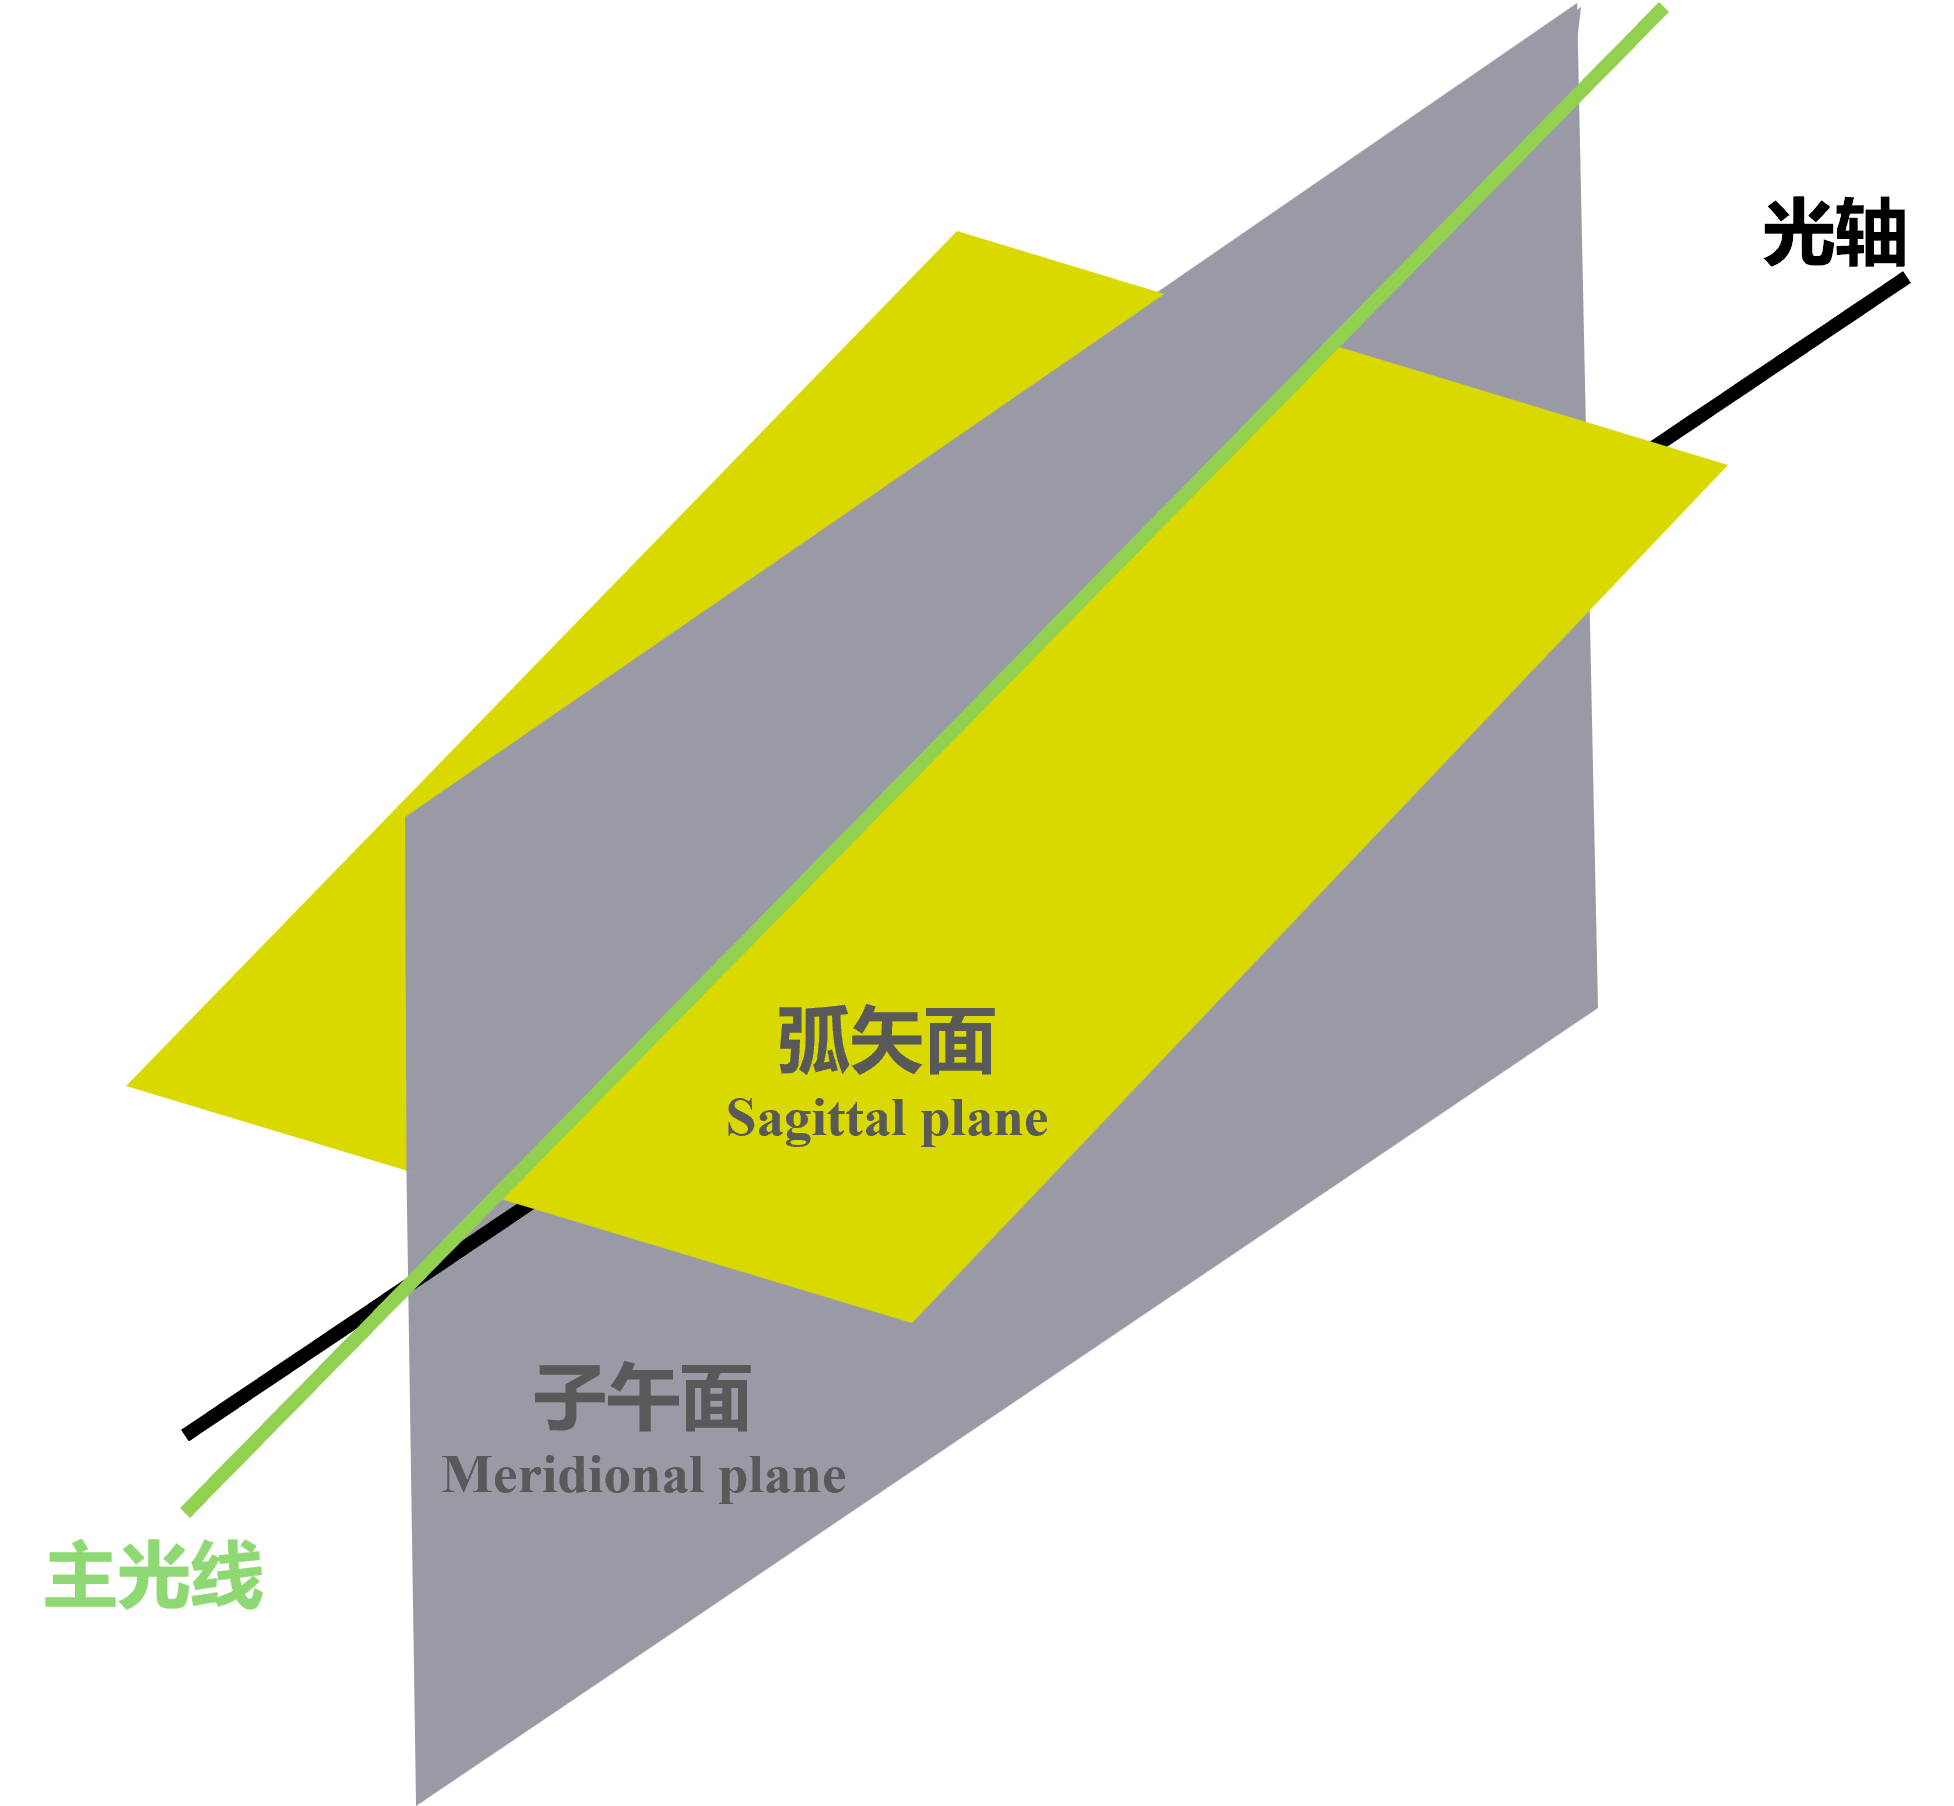
\includegraphics[width=0.9\textwidth]{Figure/图片18.png}
                \caption{子午面和弧矢面的示意图}
                \label{fig:meridional_sagittal}
            \end{figure}
        \end{column}
        \hfill
        \begin{column}{.58\textwidth}
            \begin{itemize}
                \item \textbf{子午面：}包含物点和光轴的平面
                \item \textbf{弧矢面：}垂直于子午面且包含主光线的平面
            \end{itemize}

            \bigbreak
            \textbf{像散(Astigmatism)：}
            即使同视场角，原点附近斜率在子午面和弧矢面之间\alert{不同}——子午和弧矢成像位置不一致。

            \bigbreak
            像散乃\alert{场曲的子午分量和弧矢分量分离}的状态。两个聚焦面上均呈现\alert{线像}而非点像。
        \end{column}
    \end{columns}
\end{frame}

\englishtitle{Astigmatism: Imaging and Correction}
\begin{frame}{像散成像与矫正}
    \begin{columns}[T]
        \begin{column}{.50\textwidth}
            \begin{figure}
                \centering
                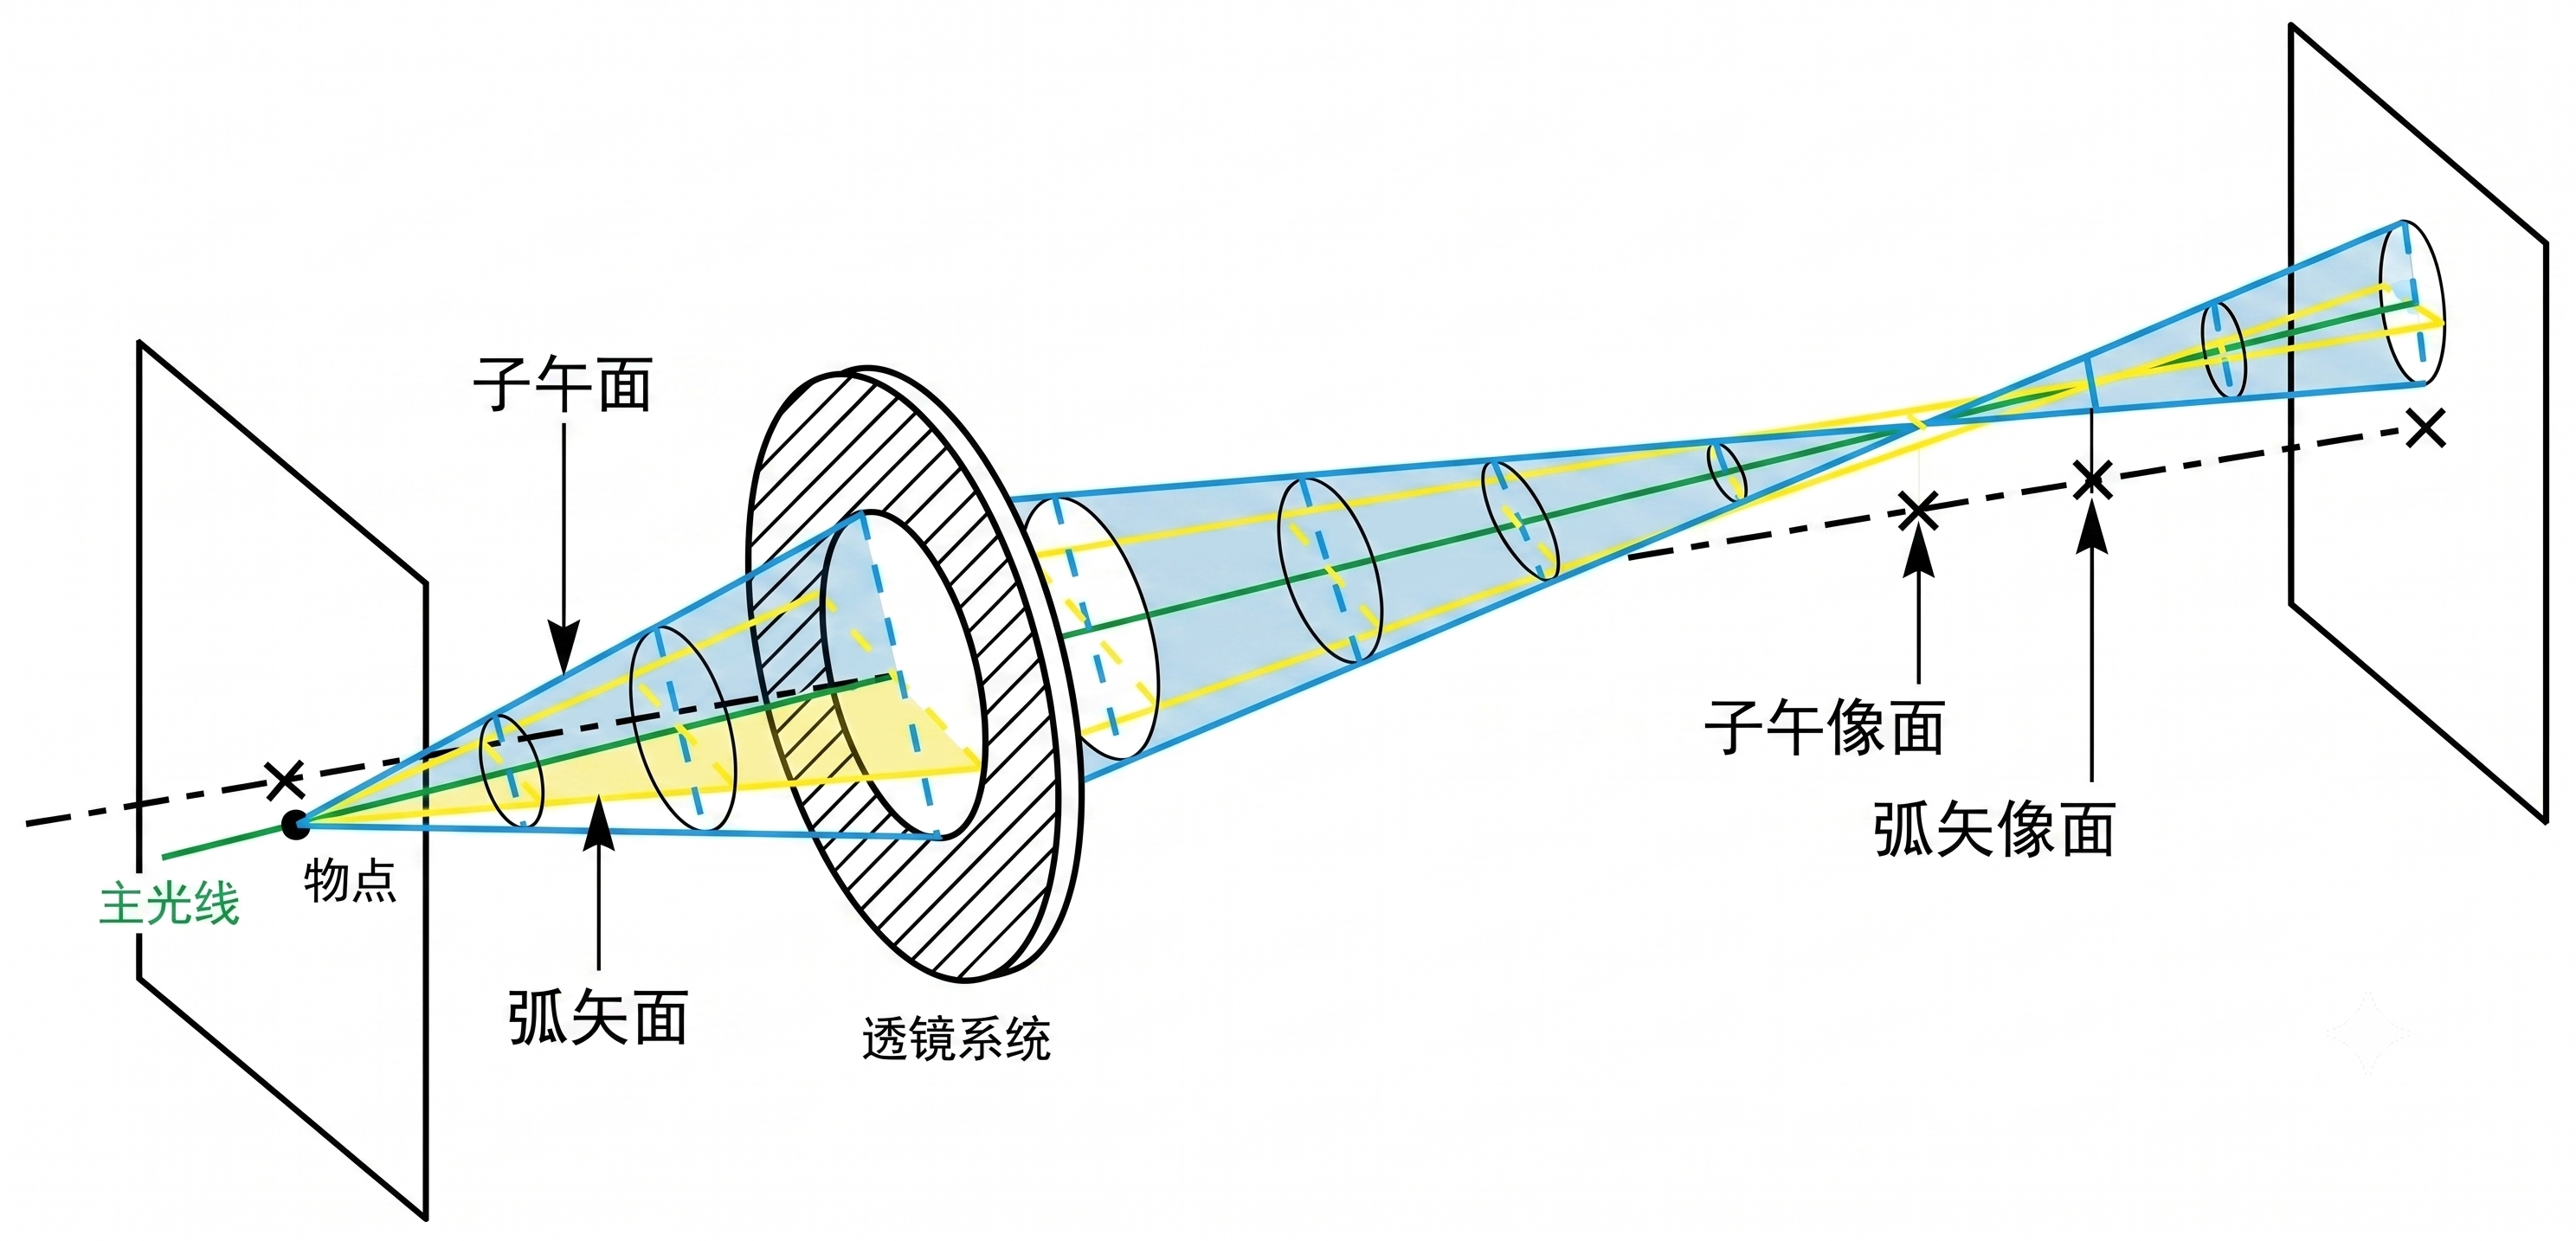
\includegraphics[width=\textwidth]{Figure/图片19.png}
                \caption{像散发生时的光路图}
                \label{fig:astigmatism_ray}
            \end{figure}
        \end{column}
        \hfill
        \begin{column}{.50\textwidth}
            \textbf{像散的本质：}
            \begin{itemize}
                \item 子午聚焦面上，弧矢光线尚未聚焦
                \item 弧矢聚焦面上，子午光线已开始发散
            \end{itemize}

            \textbf{像散矫正策略：}
            \begin{enumerate}
                \item \alert{改变光阑位置}：改变轴外光束入射对称性
                \item \alert{非球面透镜}：同时改变两方向光焦度分布
                \item \alert{对称光学结构}：前后对称自然抵消像散
            \end{enumerate}

            \alert{关键：}存在最佳光阑位置使像散为零。这与场曲不同——场曲与光阑位置无关。
        \end{column}
    \end{columns}
\end{frame}

\englishtitle{Distinguishing Three Types of Linear Aberrations}
\begin{frame}{三种线性像差的区分方法}
    \begin{figure}
        \centering
        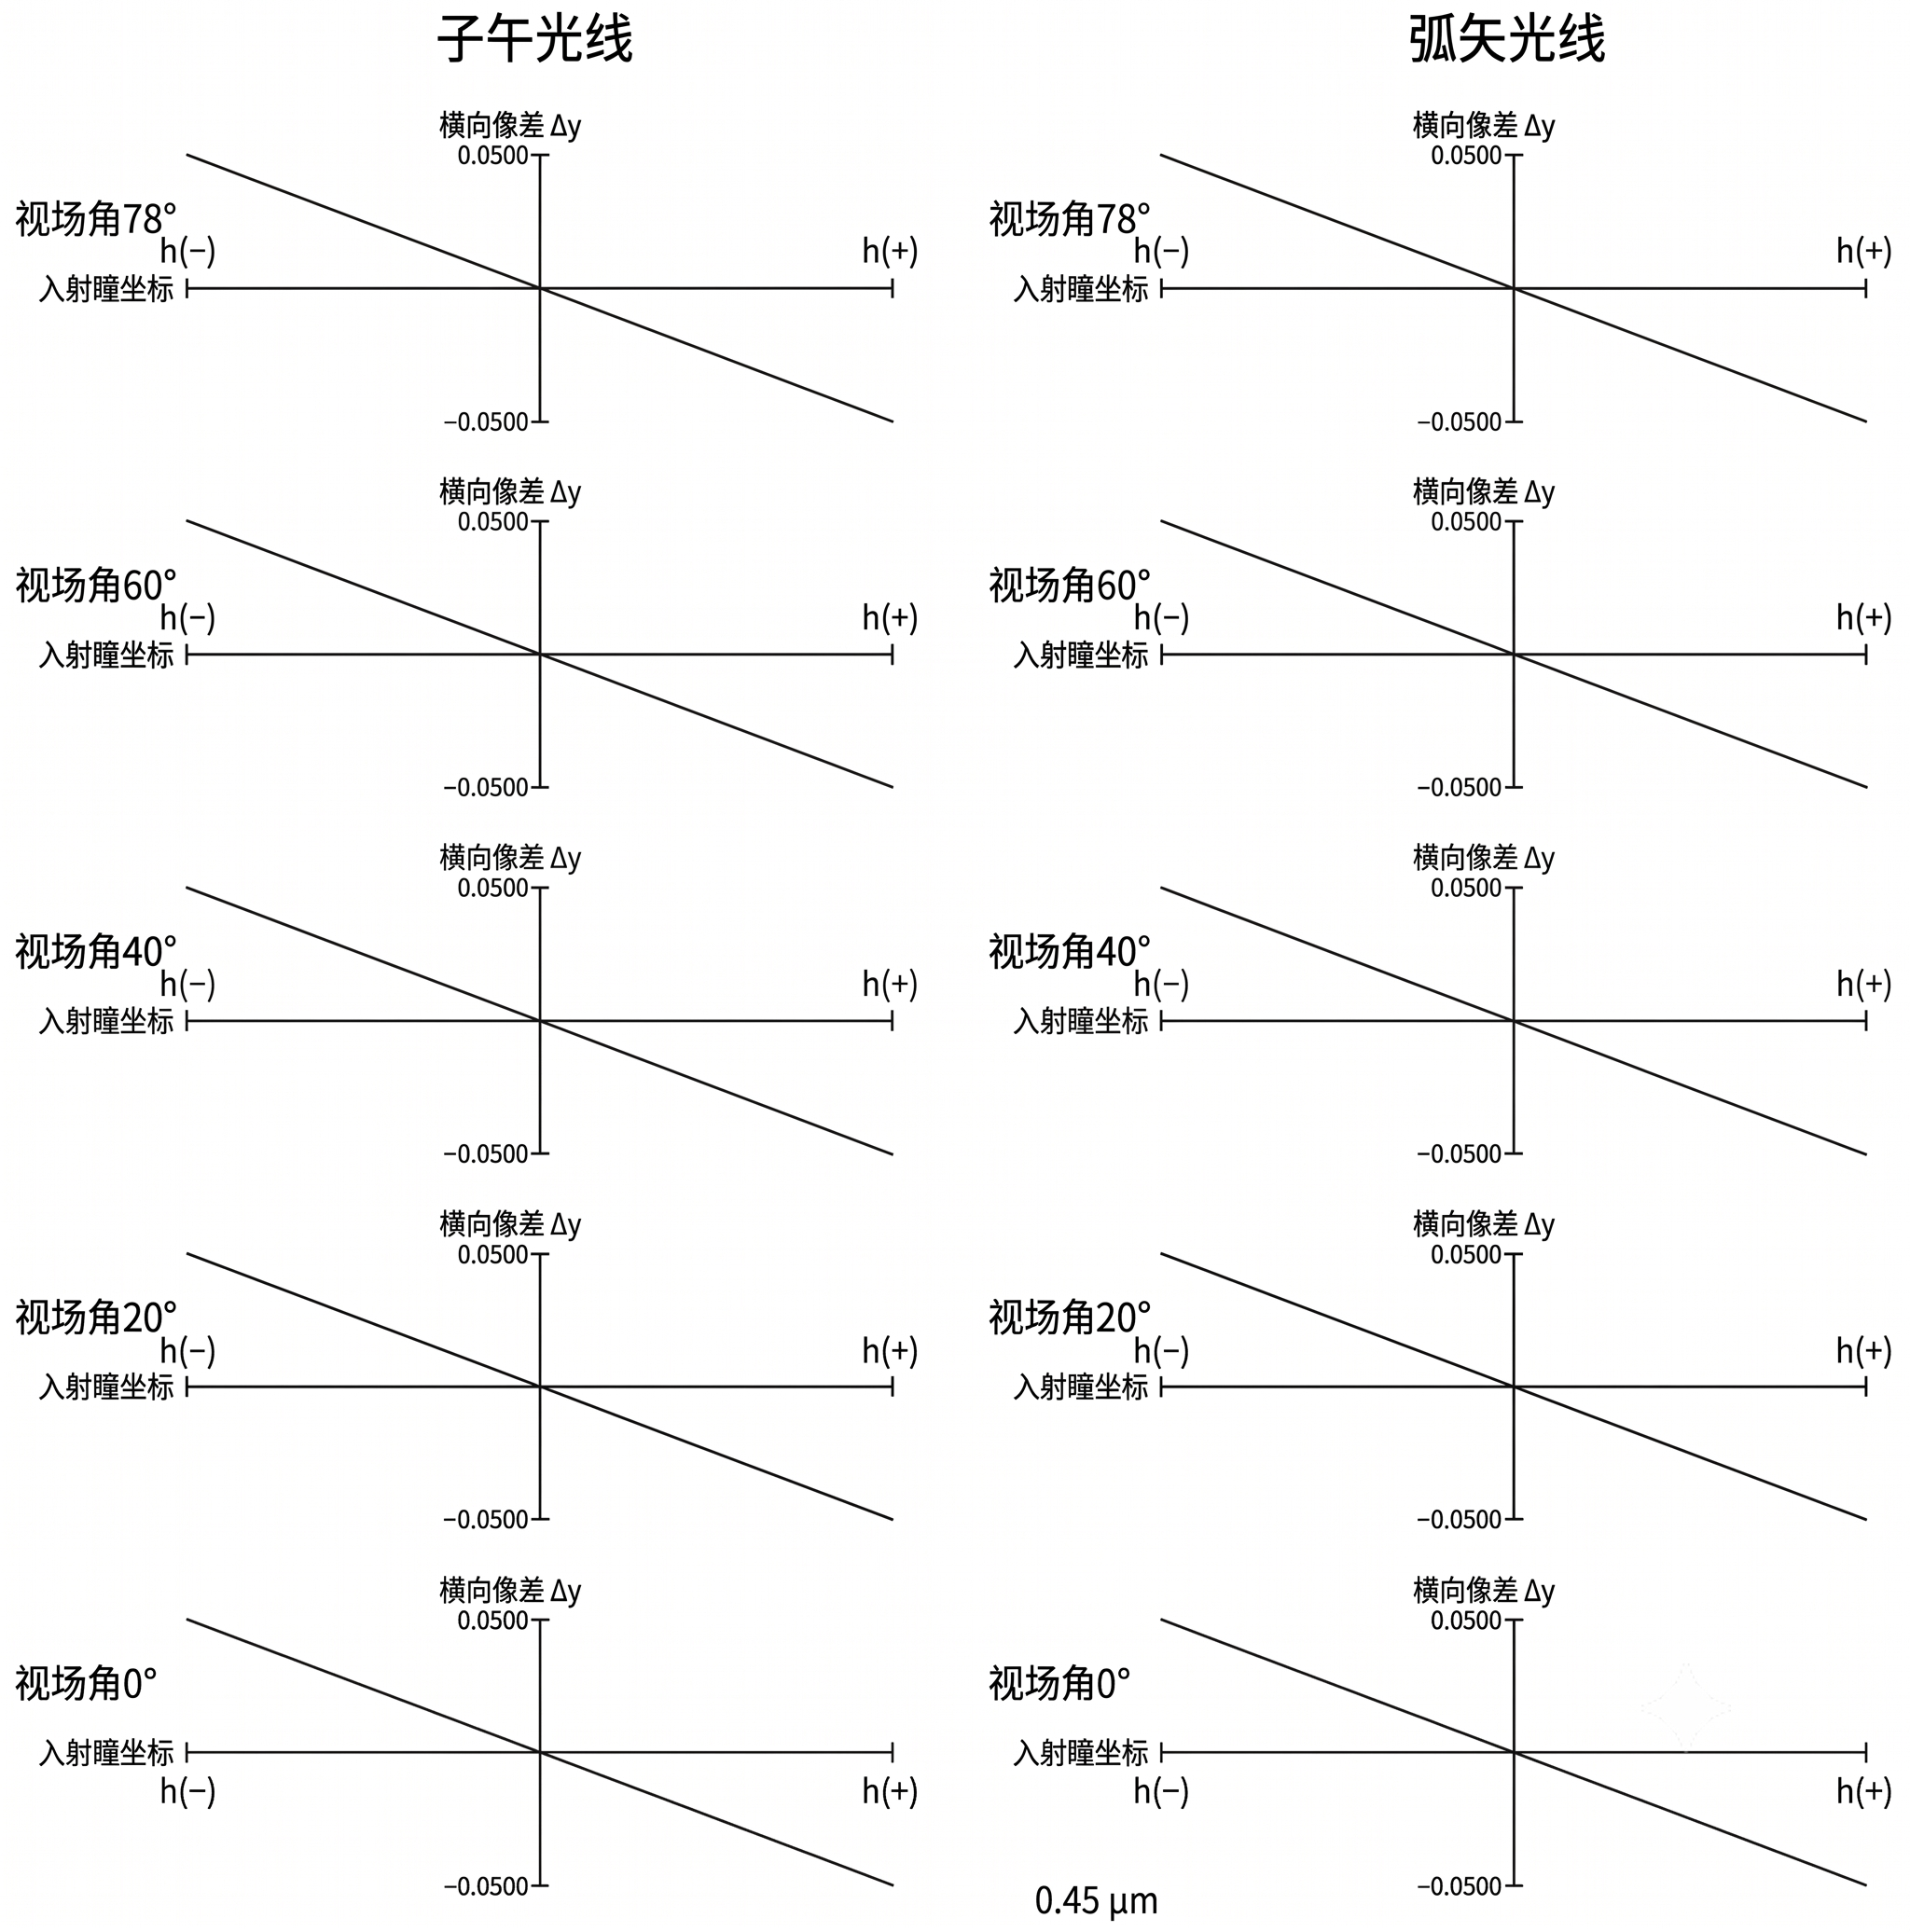
\includegraphics[width=0.3\textwidth]{Figure/图片20.png}\hfill
        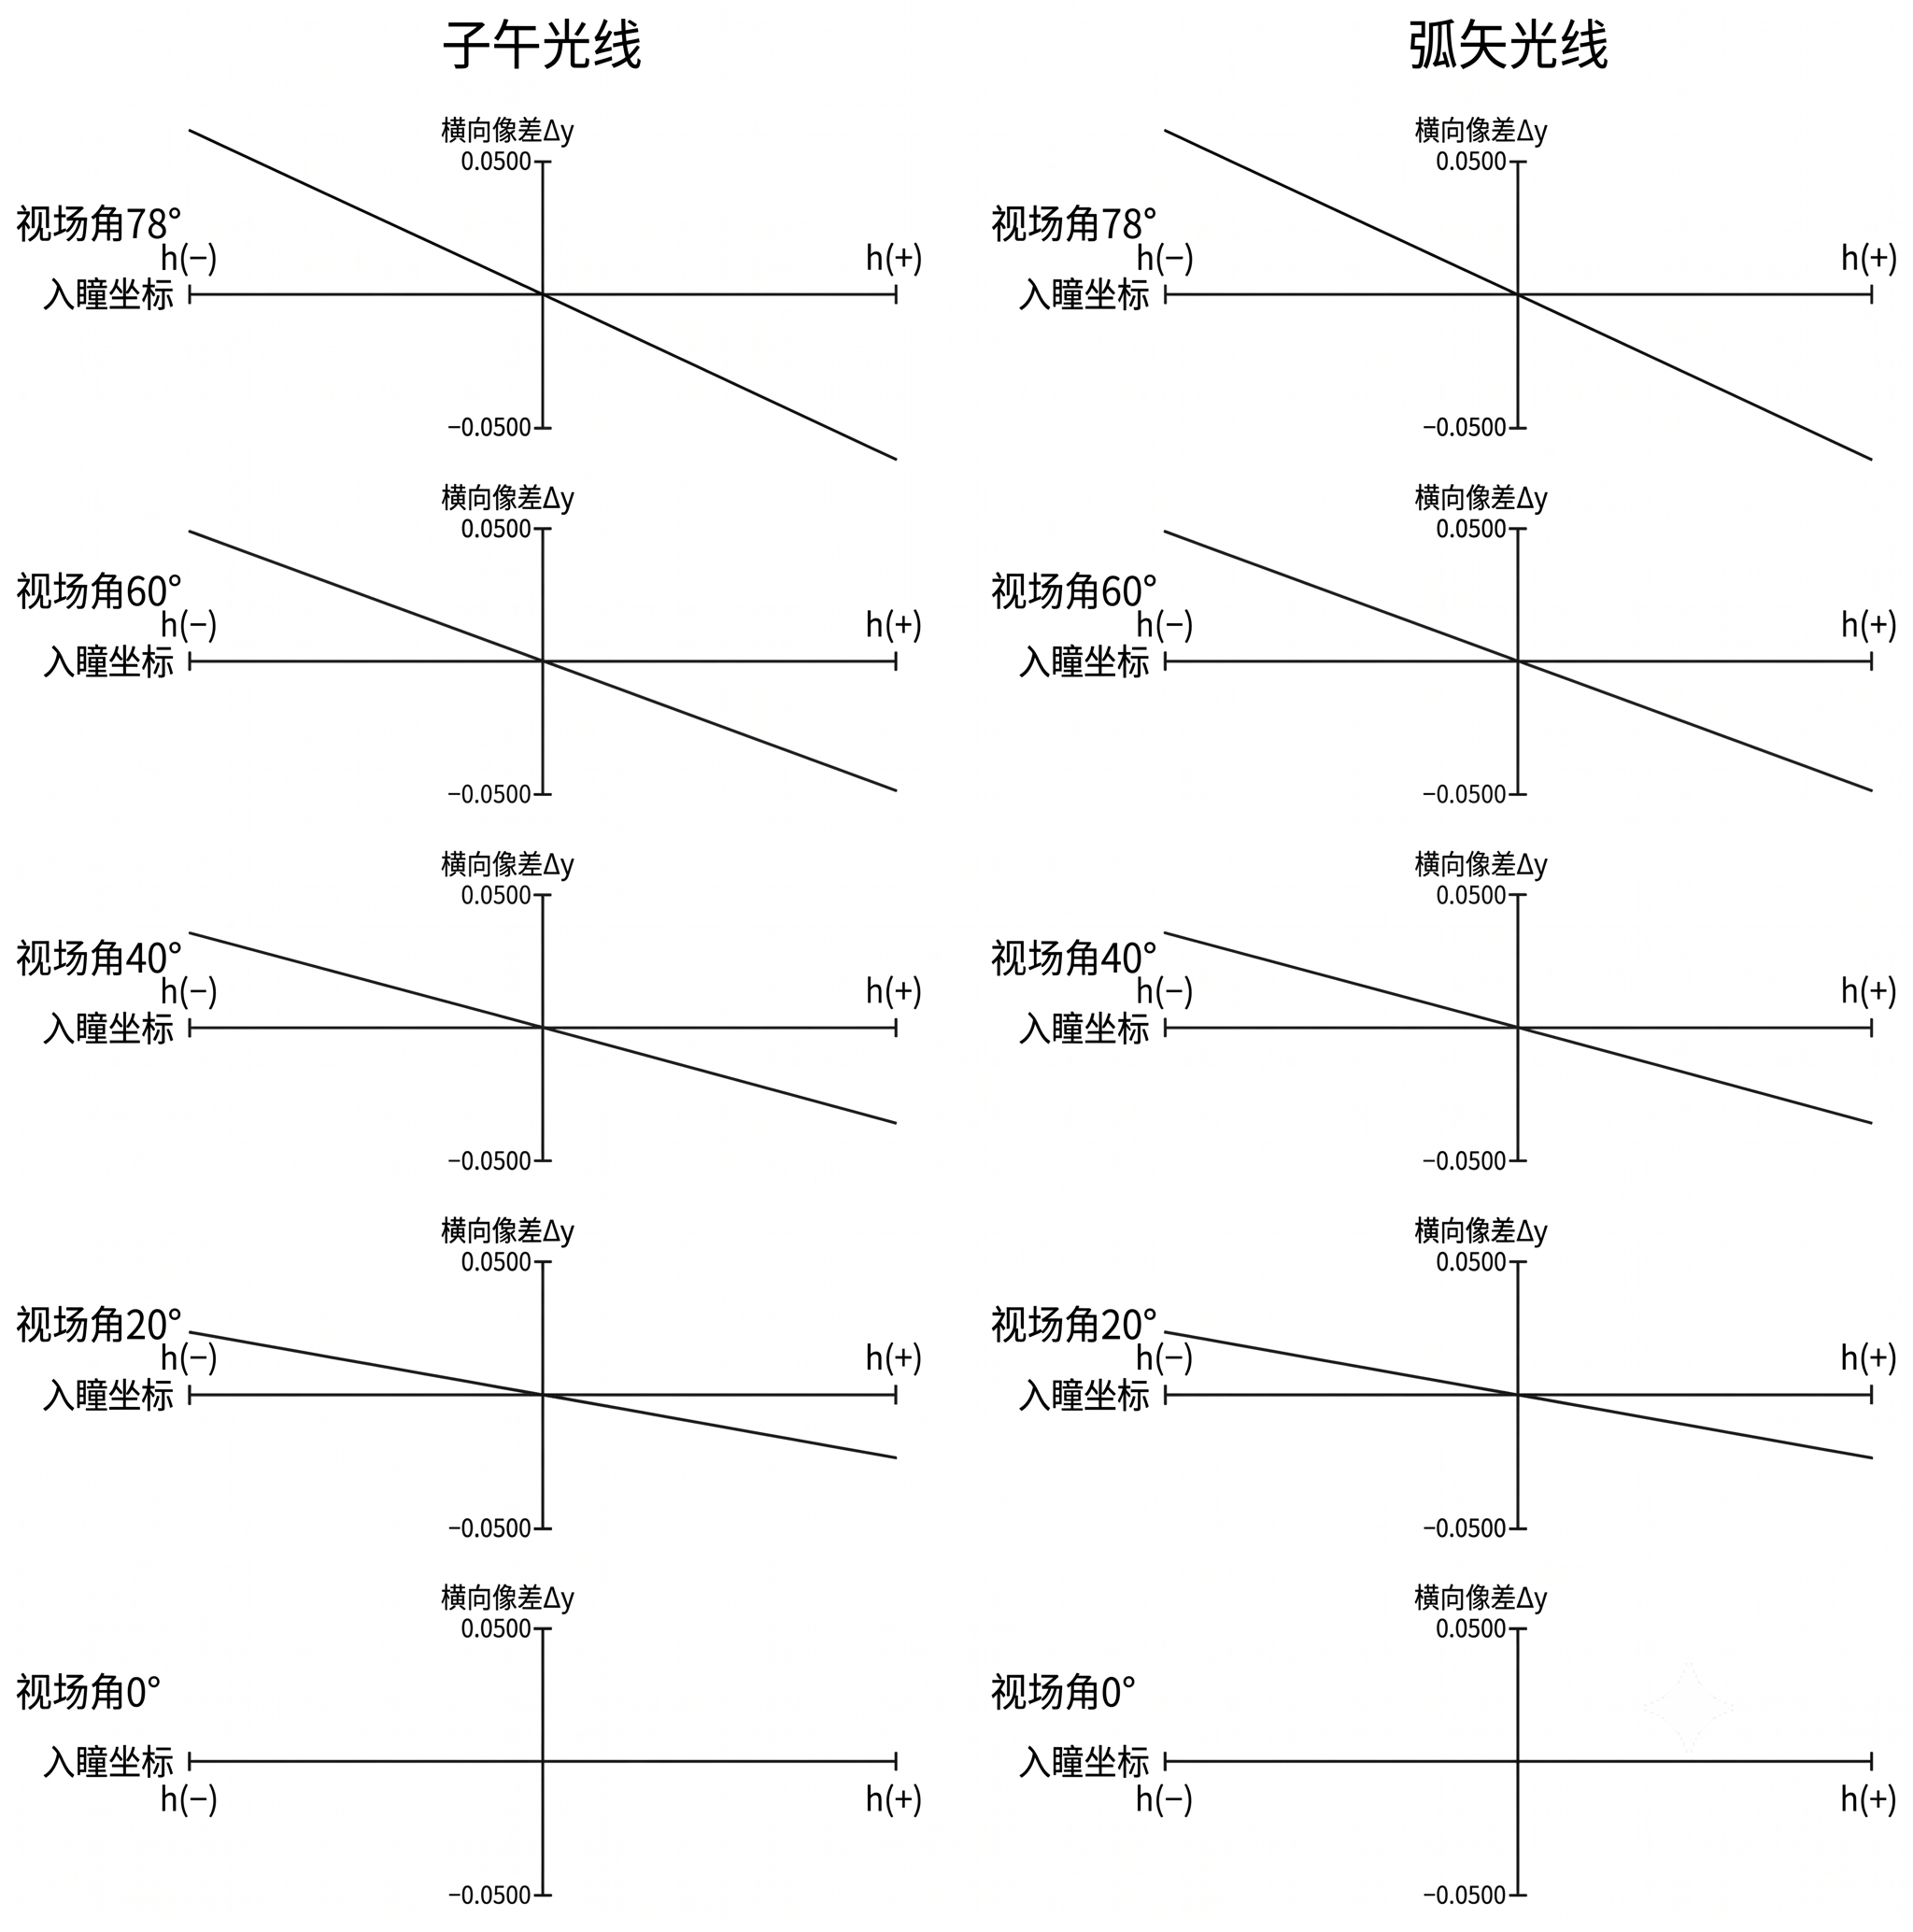
\includegraphics[width=0.3\textwidth]{Figure/图片21.png}\hfill
        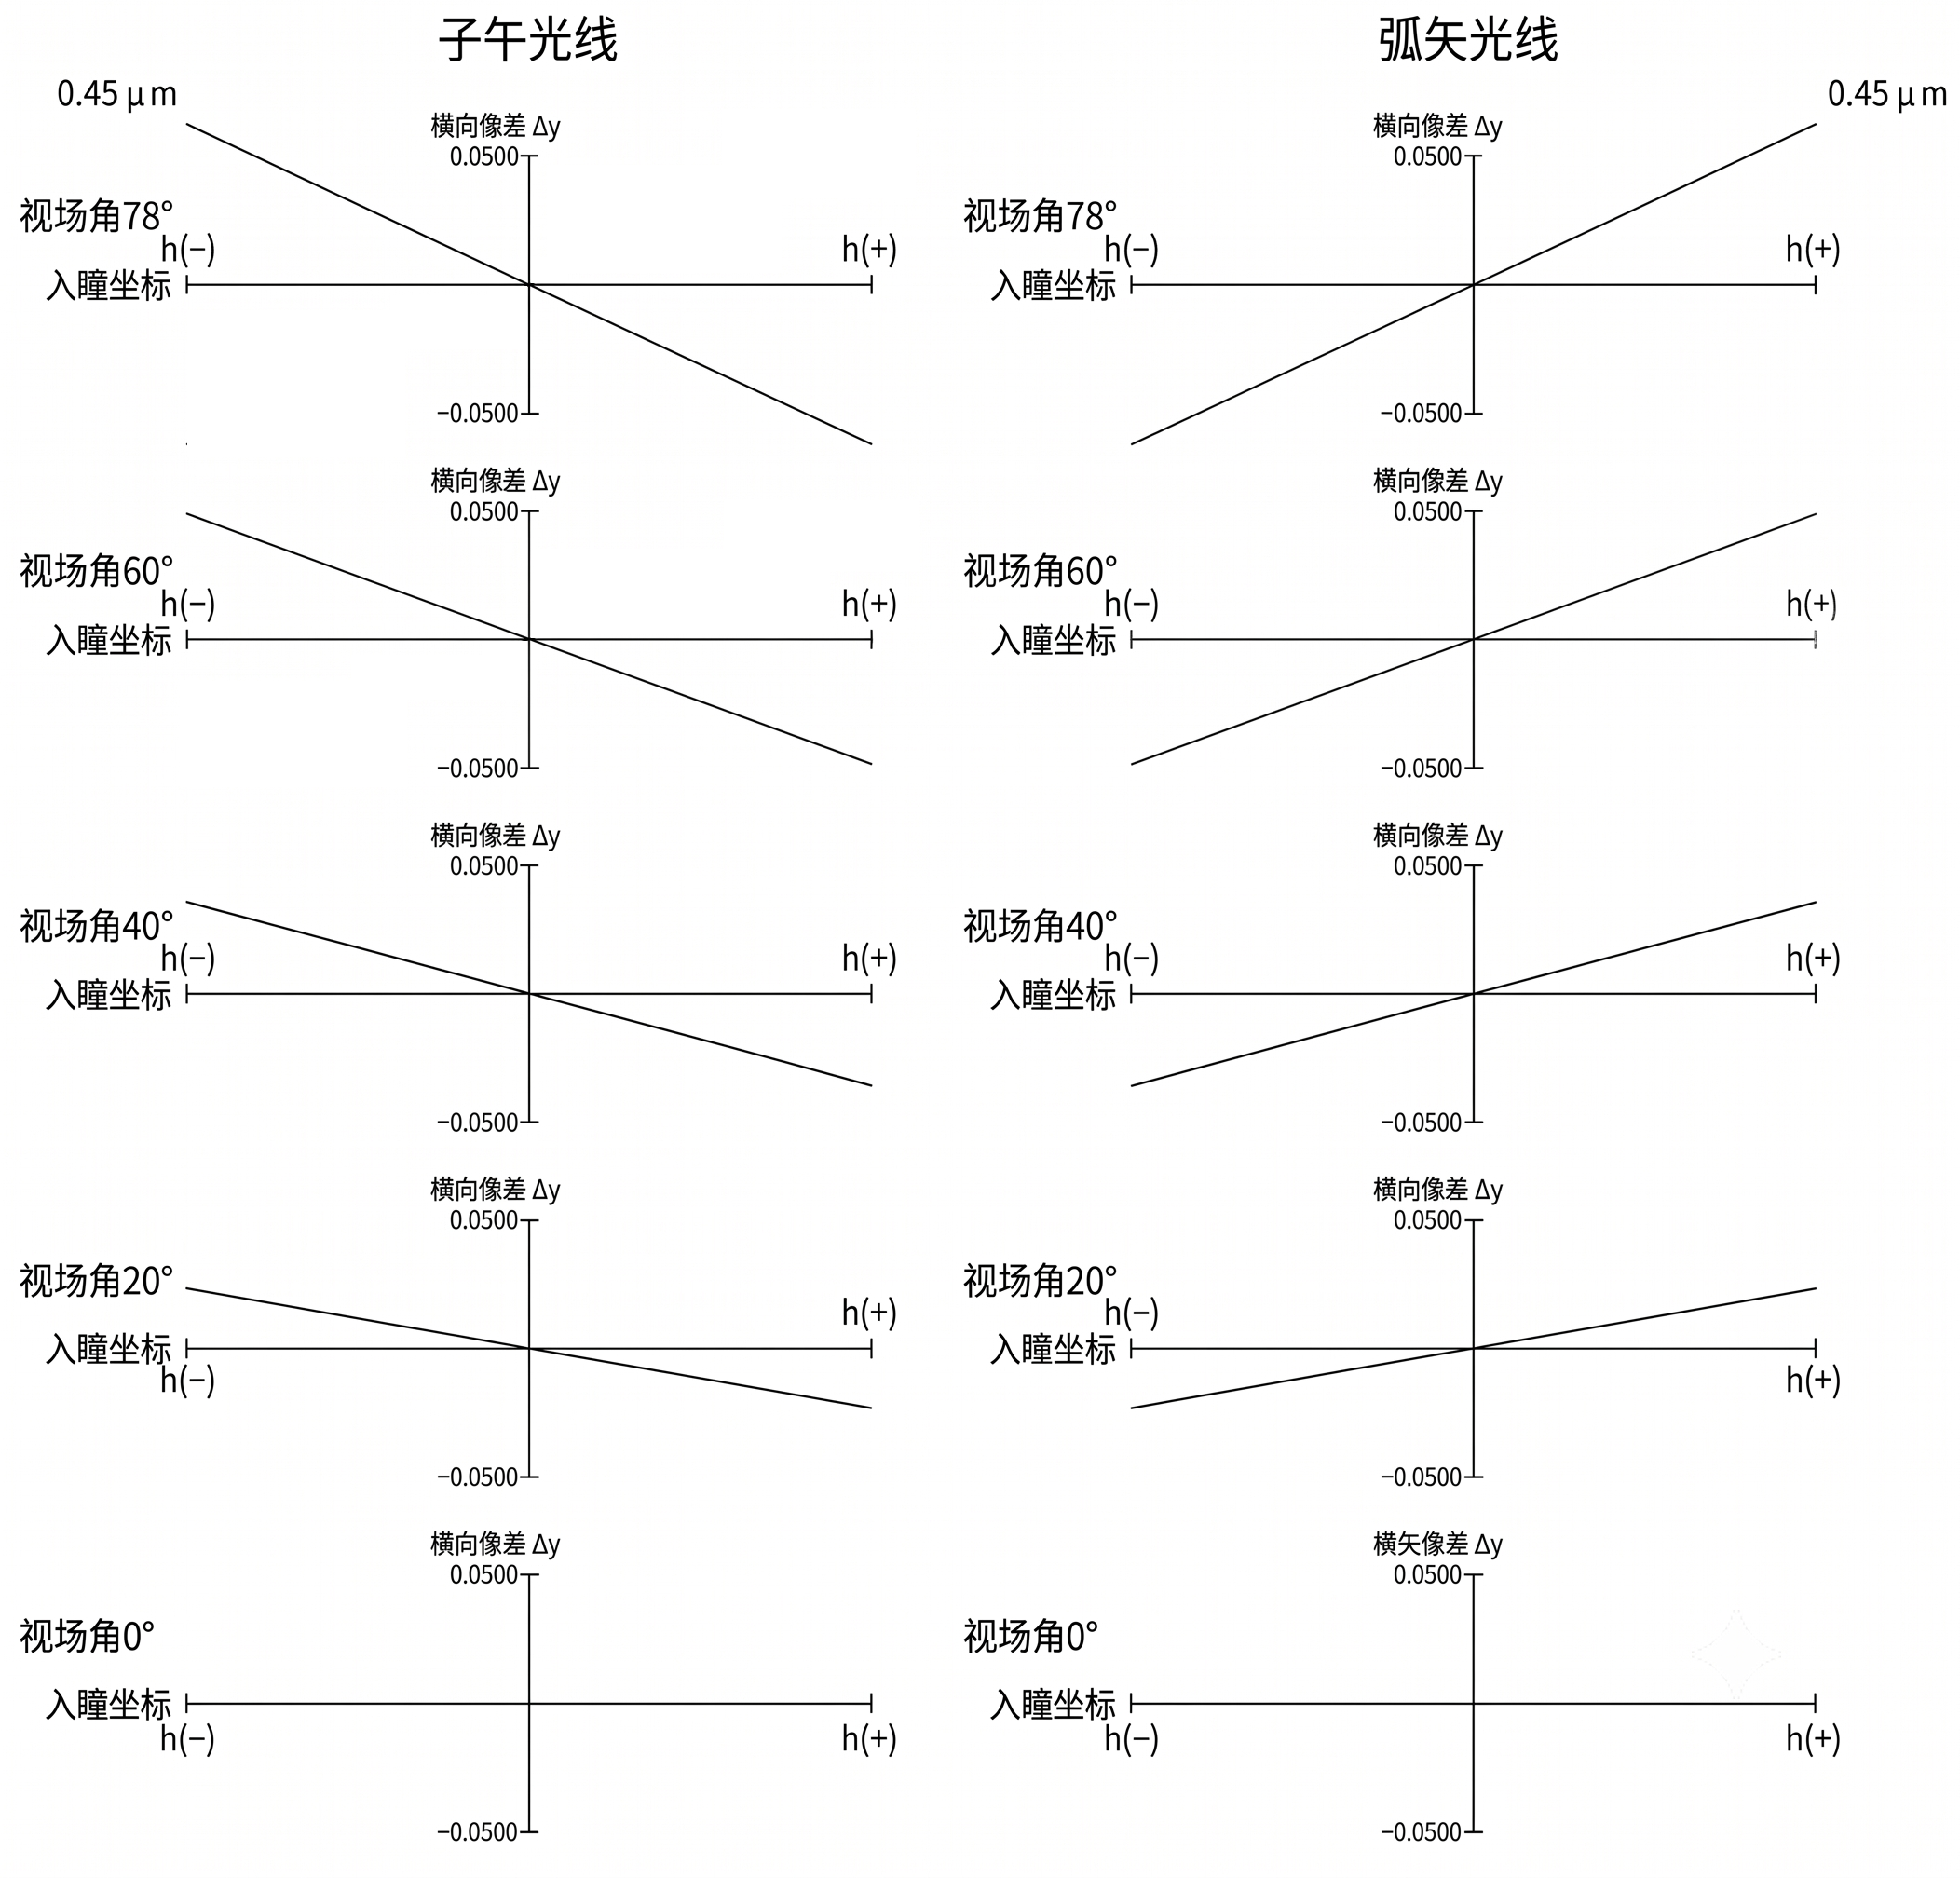
\includegraphics[width=0.3\textwidth]{Figure/图片22.png}
        \caption{离焦(左)：斜率均一\quad 场曲(中)：子午/弧矢一致\quad 像散(右)：子午/弧矢不同}
        \label{fig:linear_distinction}
    \end{figure}

    \smallbreak
    \begin{table}
        \centering
        \begin{tabular}{c|c|c}
            \toprule
            \textbf{像差类型} & \textbf{斜率与视场角关系} & \textbf{子午与弧矢关系} \\
            \midrule
            离焦 & 均一           & 一致 \\
            场曲 & 因视场角而异   & 一致 \\
            像散 & 因视场角而异   & \alert{不一致} \\
            \bottomrule
        \end{tabular}
        \caption{离焦、场曲与像散的区分准则}
        \label{tab:linear_aberration}
    \end{table}
\end{frame}

\subsection{色差、渐晕与衍射极限}

\englishtitle{Vignetting and Pupil Aberration}
\begin{frame}{渐晕与光瞳像差}
    \begin{columns}[T]
        \begin{column}{.45\textwidth}
            \begin{figure}
                \centering
                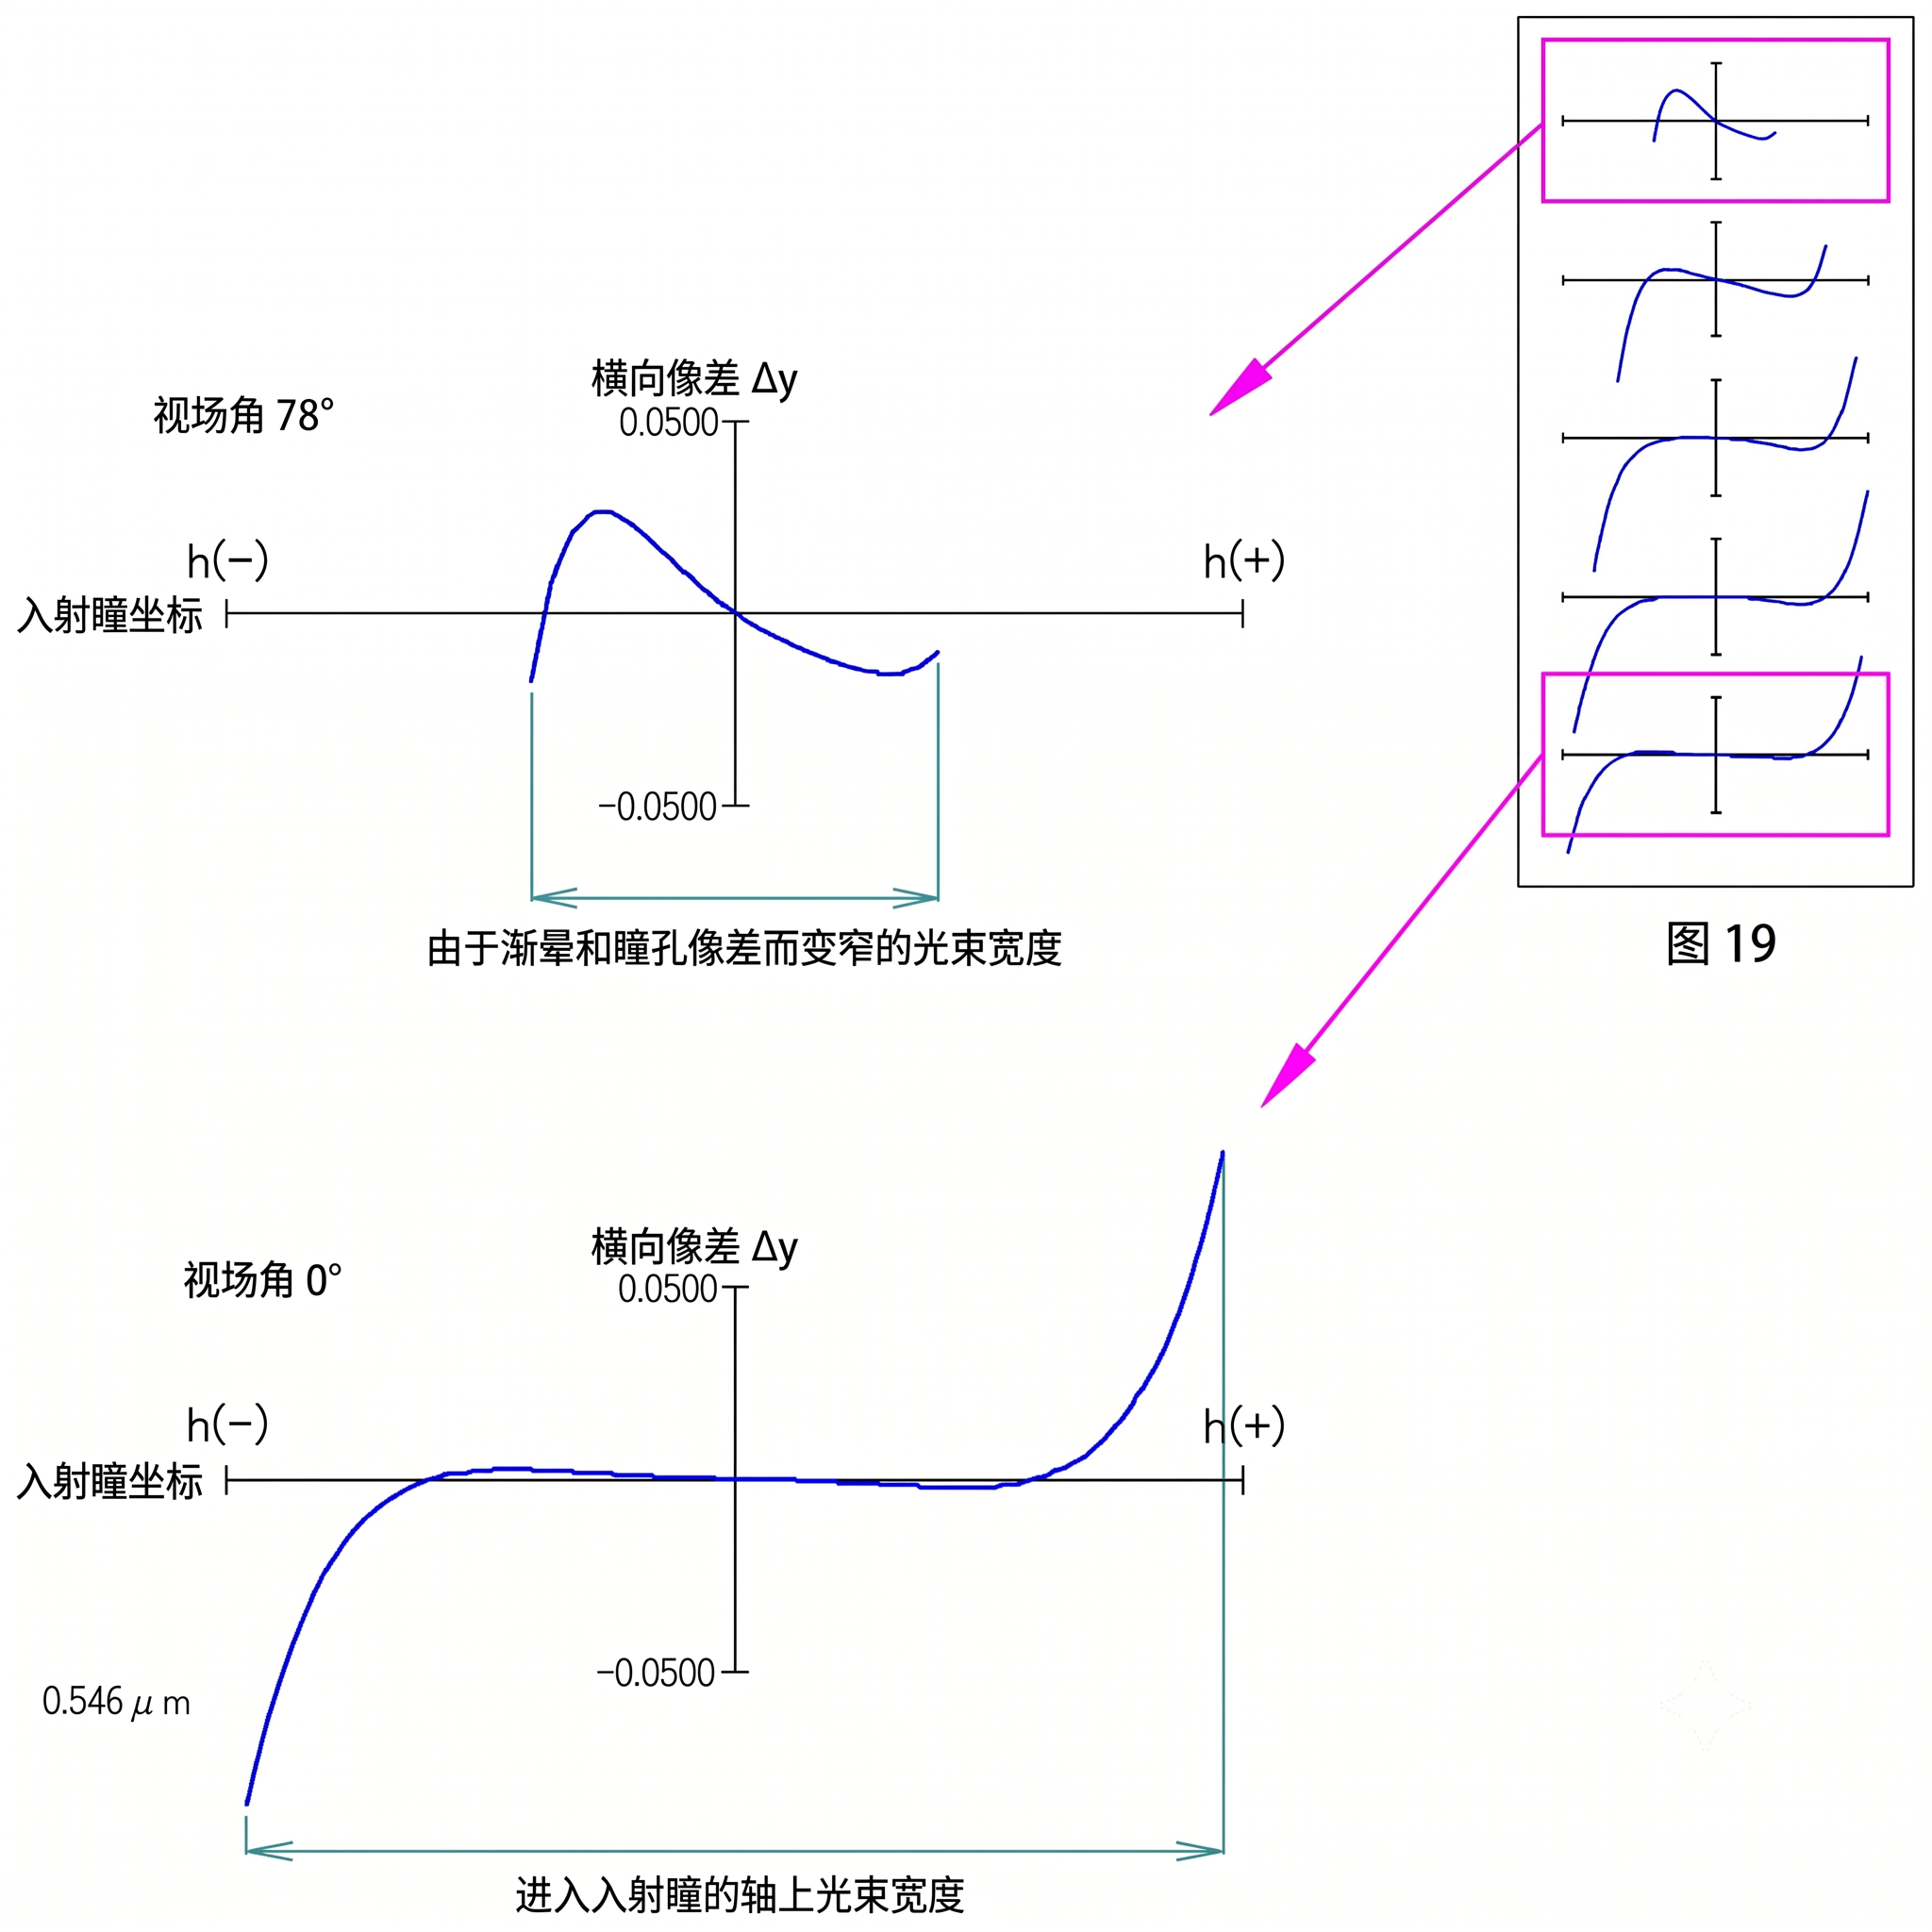
\includegraphics[width=0.9\textwidth]{Figure/图片27.png}
                \caption{渐晕和光瞳像差引起宽度差异}
                \label{fig:vignetting}
            \end{figure}
        \end{column}
        \hfill
        \begin{column}{.55\textwidth}
            比较 $0^\circ$ 和 $78^\circ$ 视场角的横向像差图，轴外光束宽度\alert{更窄}。

            \bigbreak
            \begin{itemize}
                \item \alert{渐晕(Vignetting)}：大视场下镜筒或透镜边缘遮挡光束
                \item \alert{光瞳像差}：轴上与轴外光束形成的入瞳形状不同
            \end{itemize}

            \textbf{判断方法：}比较满刻度(近轴入瞳直径)与实际宽度。
            \alert{注意：}入瞳直径是近轴量，不受渐晕影响。
        \end{column}
    \end{columns}
\end{frame}

\englishtitle{Axial Chromatic Aberration}
\begin{frame}{轴向色差}
    \begin{columns}[T]
        \begin{column}{.46\textwidth}
            \begin{figure}
                \centering
                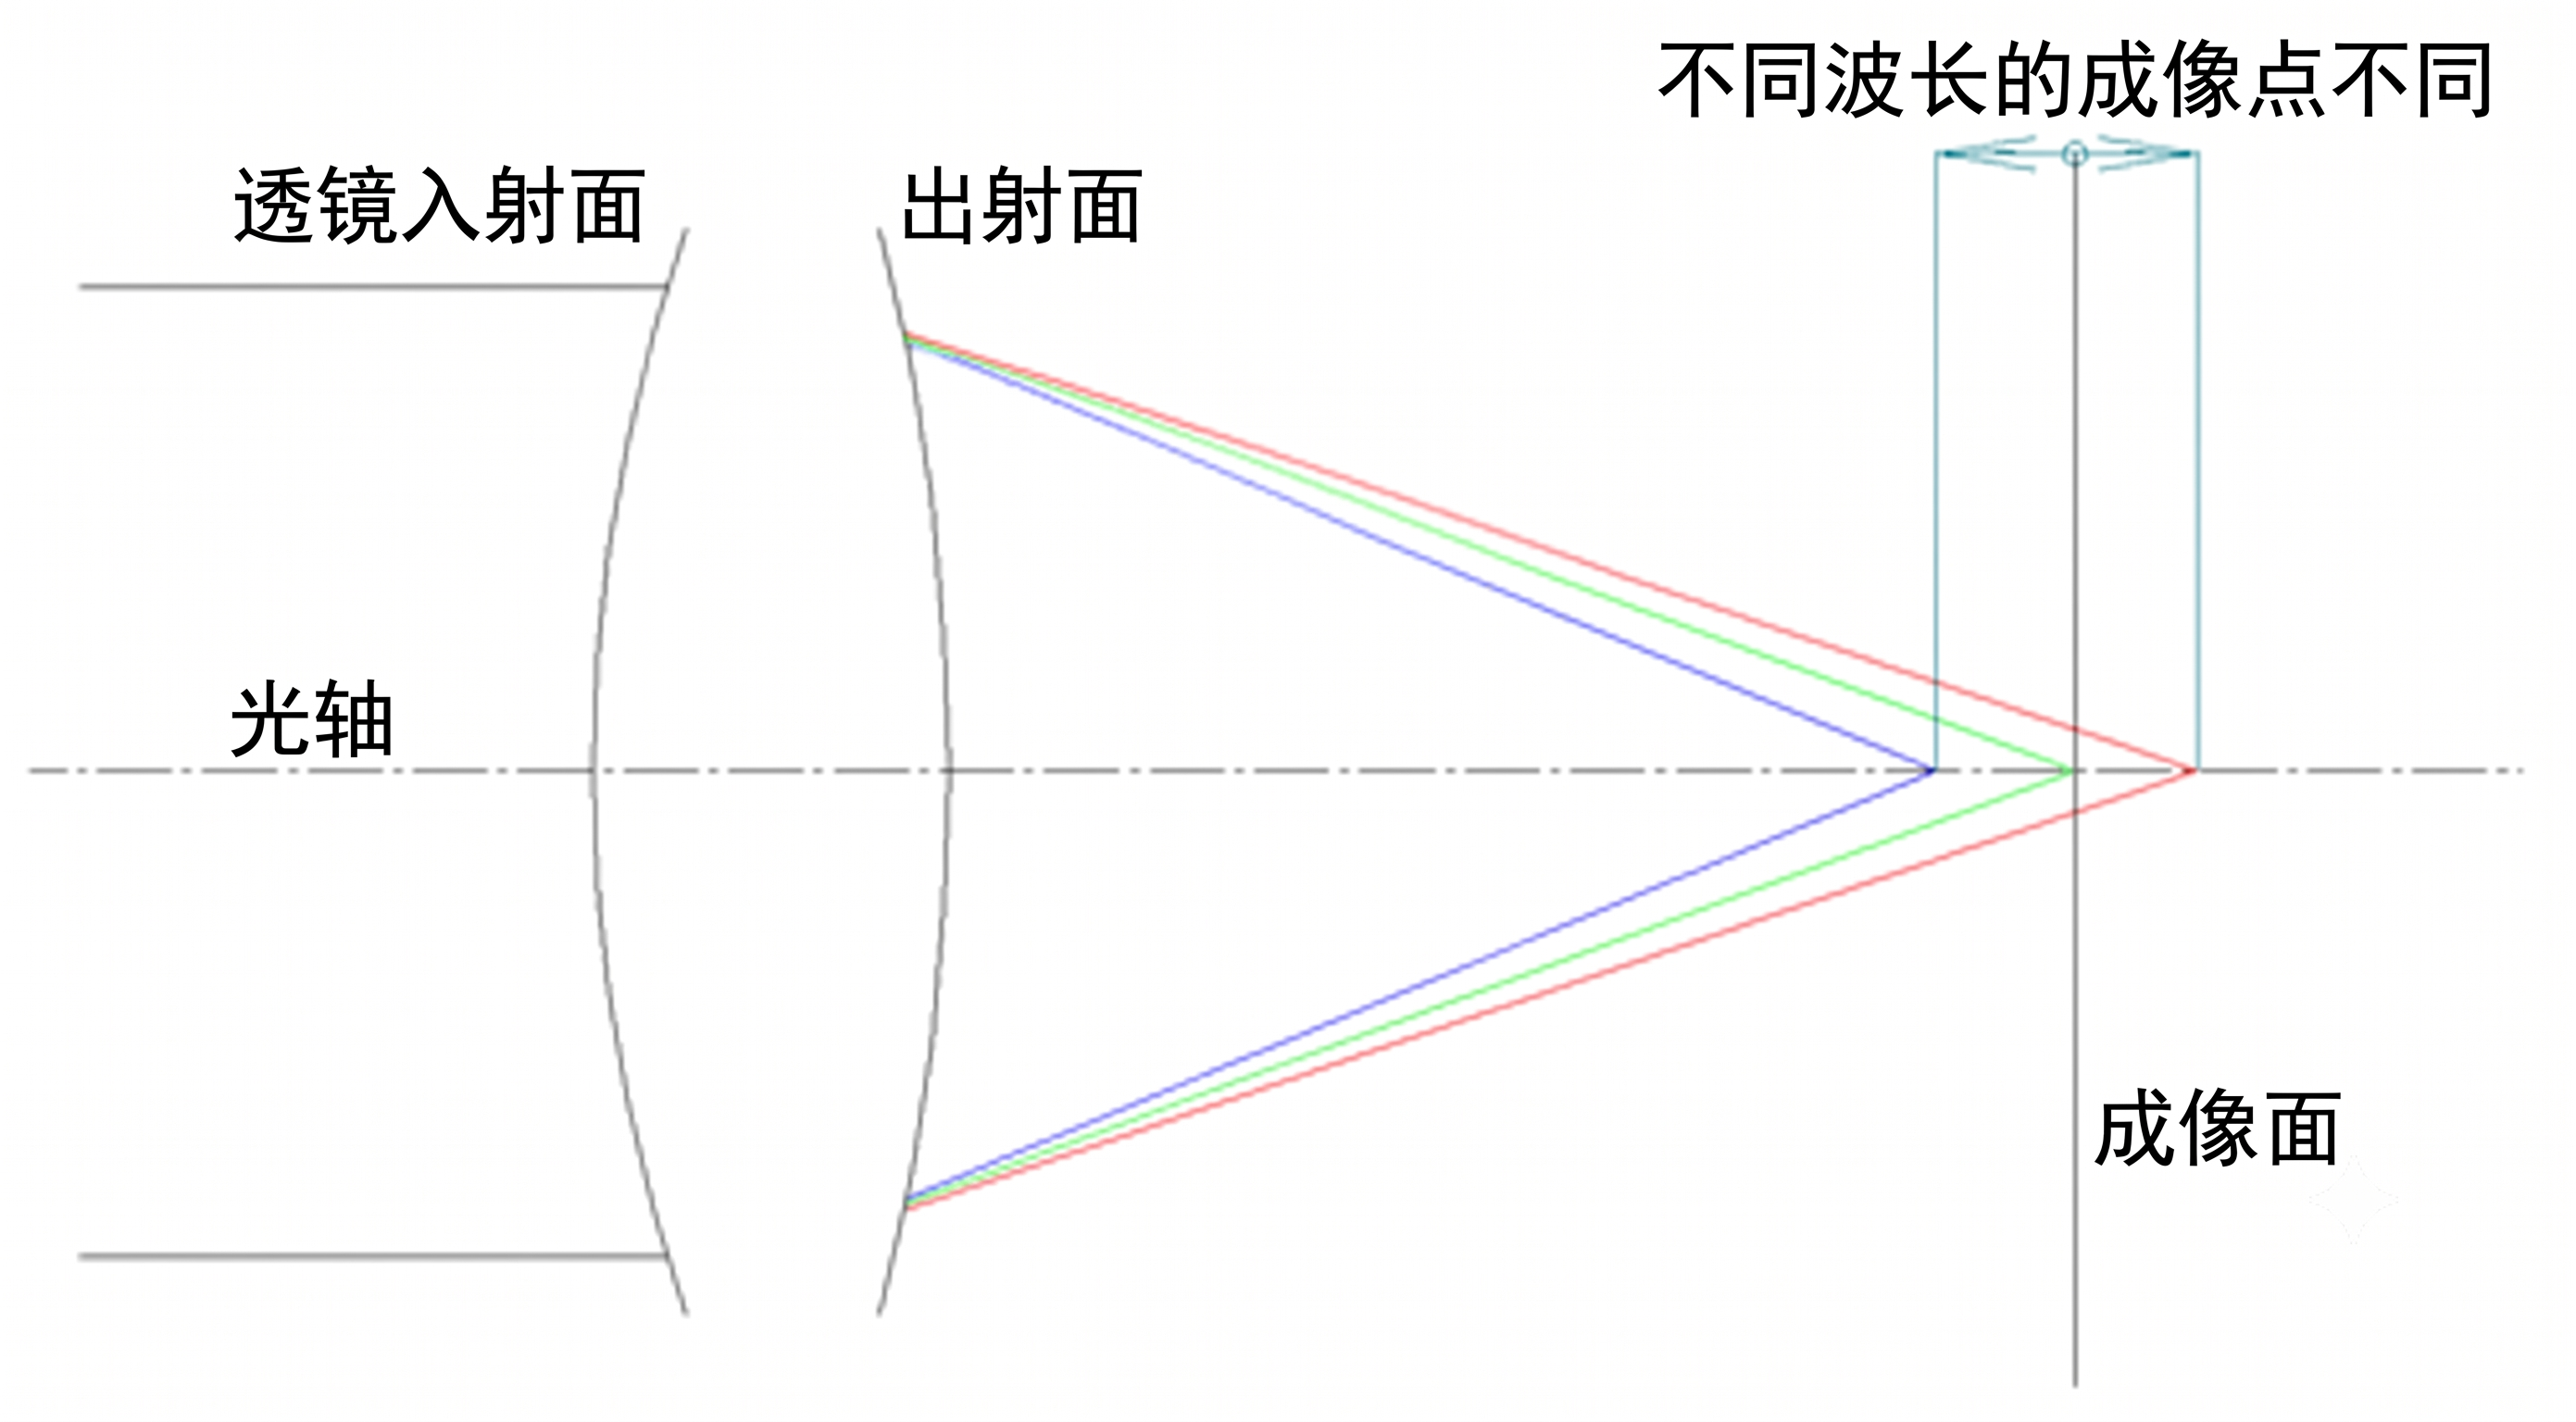
\includegraphics[width=0.98\textwidth]{Figure/图片30.png}\\[3pt]
                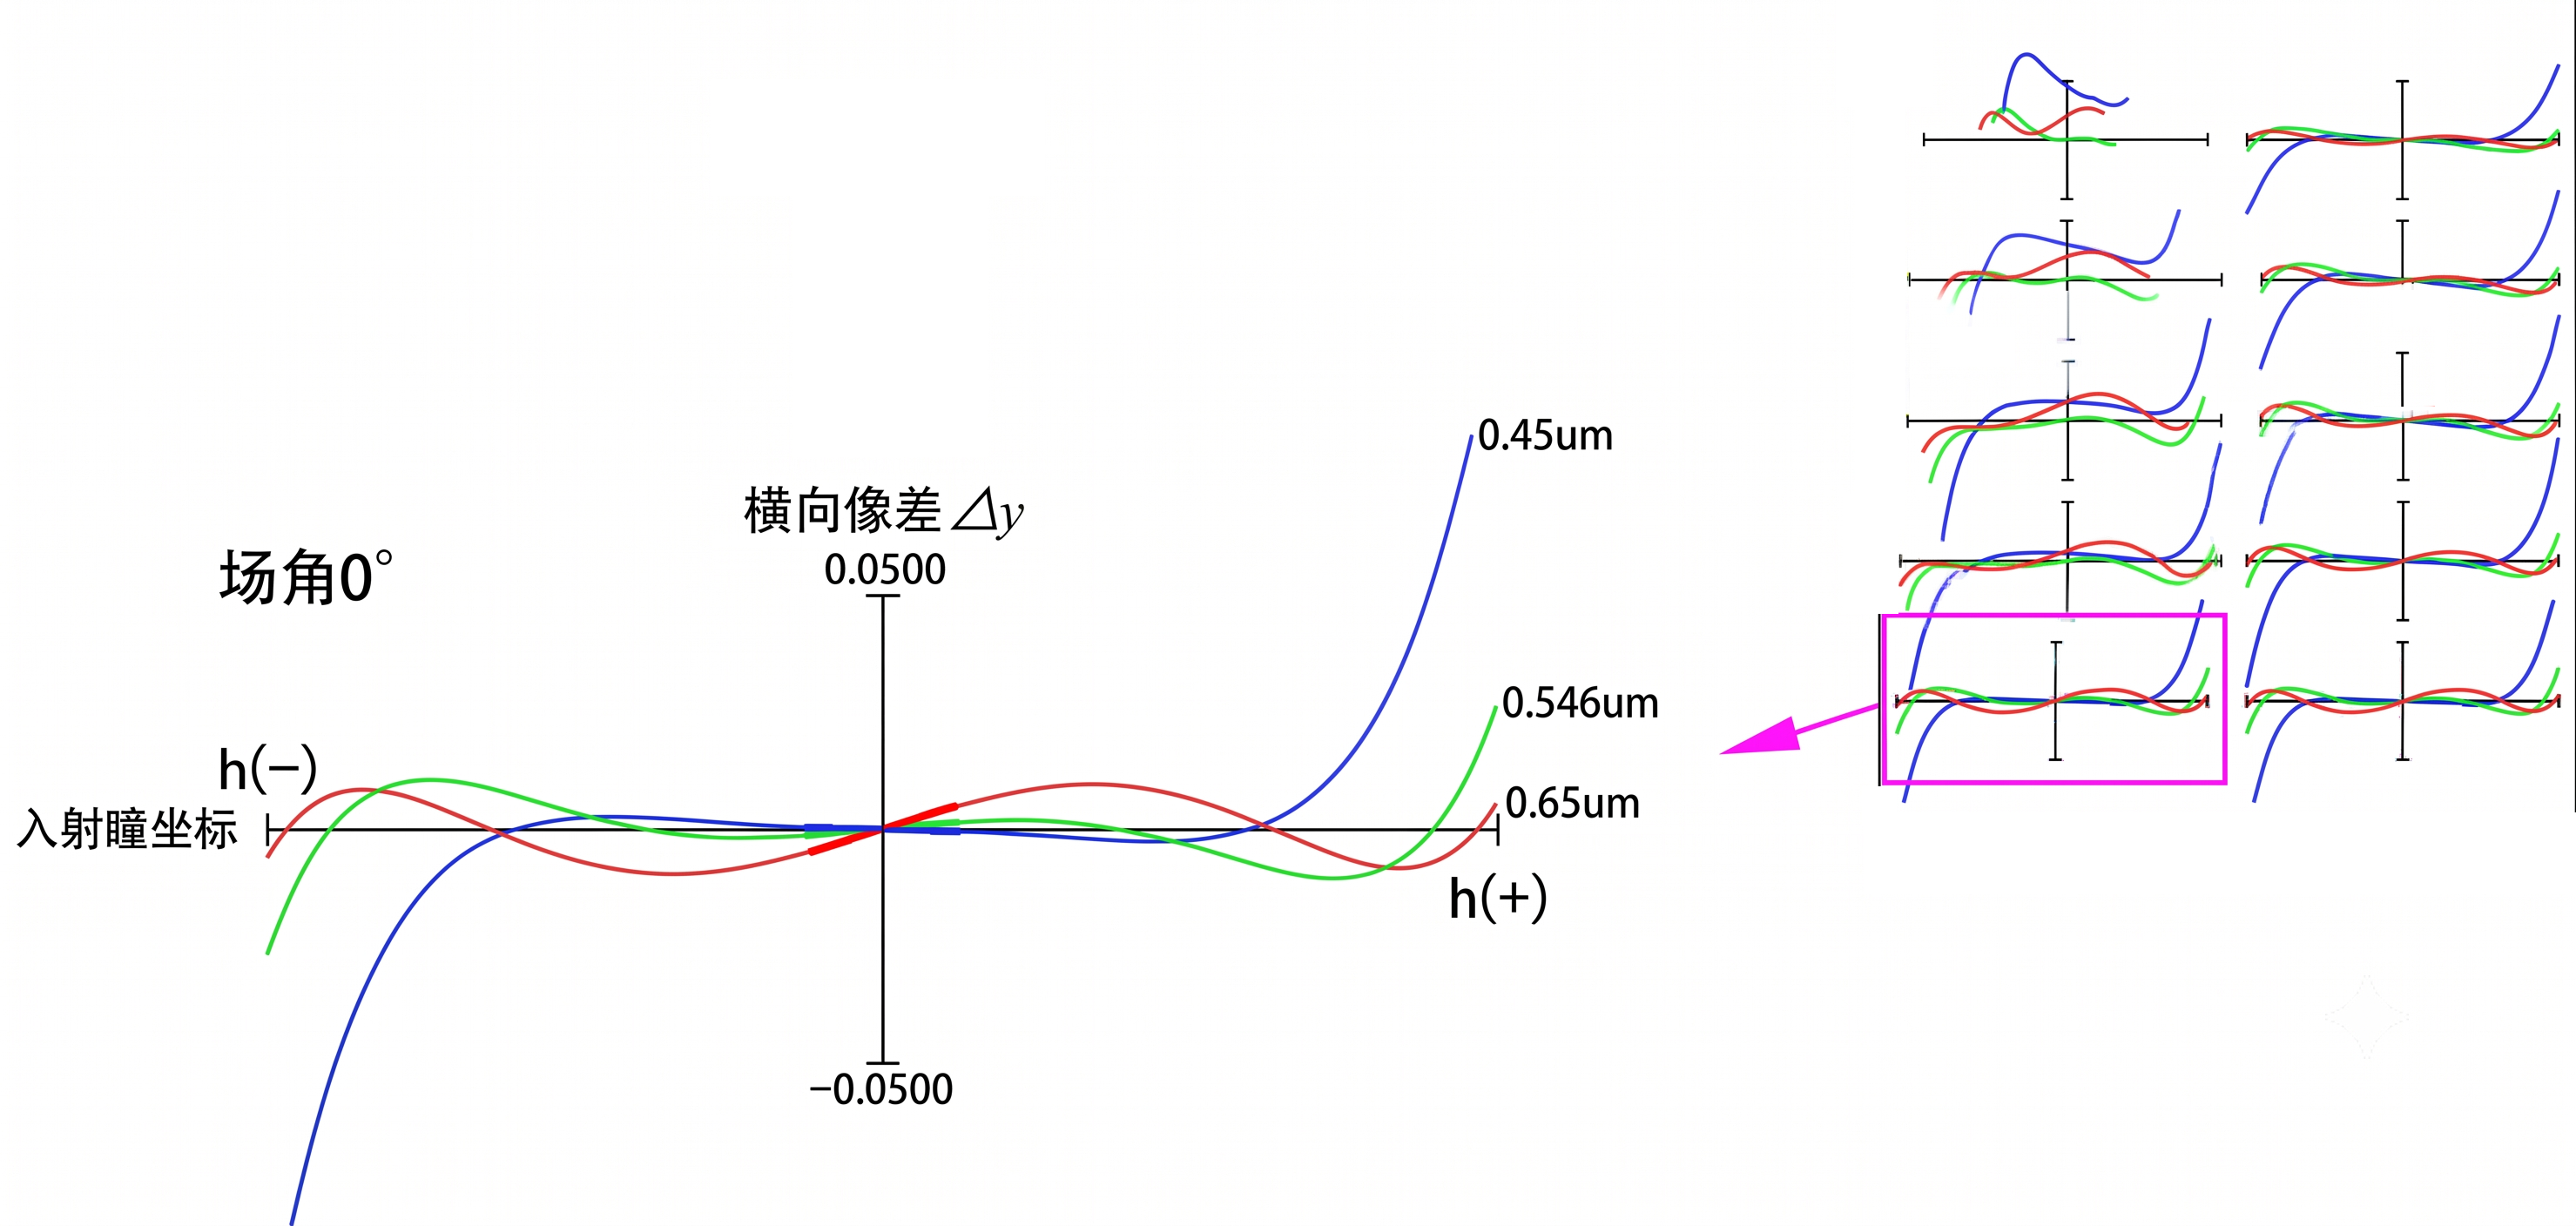
\includegraphics[width=0.98\textwidth]{Figure/图片28.png}
                \caption{轴向色差的光路示意与横向像差图特征}
                \label{fig:axial_color}
            \end{figure}
        \end{column}
        \hfill
        \begin{column}{.54\textwidth}
            \textbf{轴向色差(纵色差/位置色差)：}
            \bigbreak
            轴上光束横向像差图\alert{原点附近}斜率因波长不同——近轴像点位置具有\alert{波长依赖性}。

            \bigbreak
            \textbf{物理机制：}
            \begin{itemize}
                \item $n(\lambda)$ 随波长变化：短波折射率高，焦点近
                \item 原点附近球差($\propto h^3$)和彗差($\propto h^2$)影响最小
                \item 轴向色差($\propto h^1$)在原点附近\alert{占主导}
            \end{itemize}

            矫正：\alert{消色差双透镜(achromat)}。
        \end{column}
    \end{columns}
\end{frame}

\englishtitle{Lateral Chromatic Aberration}
\begin{frame}{倍率色差}
    \begin{columns}[T]
        \begin{column}{.46\textwidth}
            \begin{figure}
                \centering
                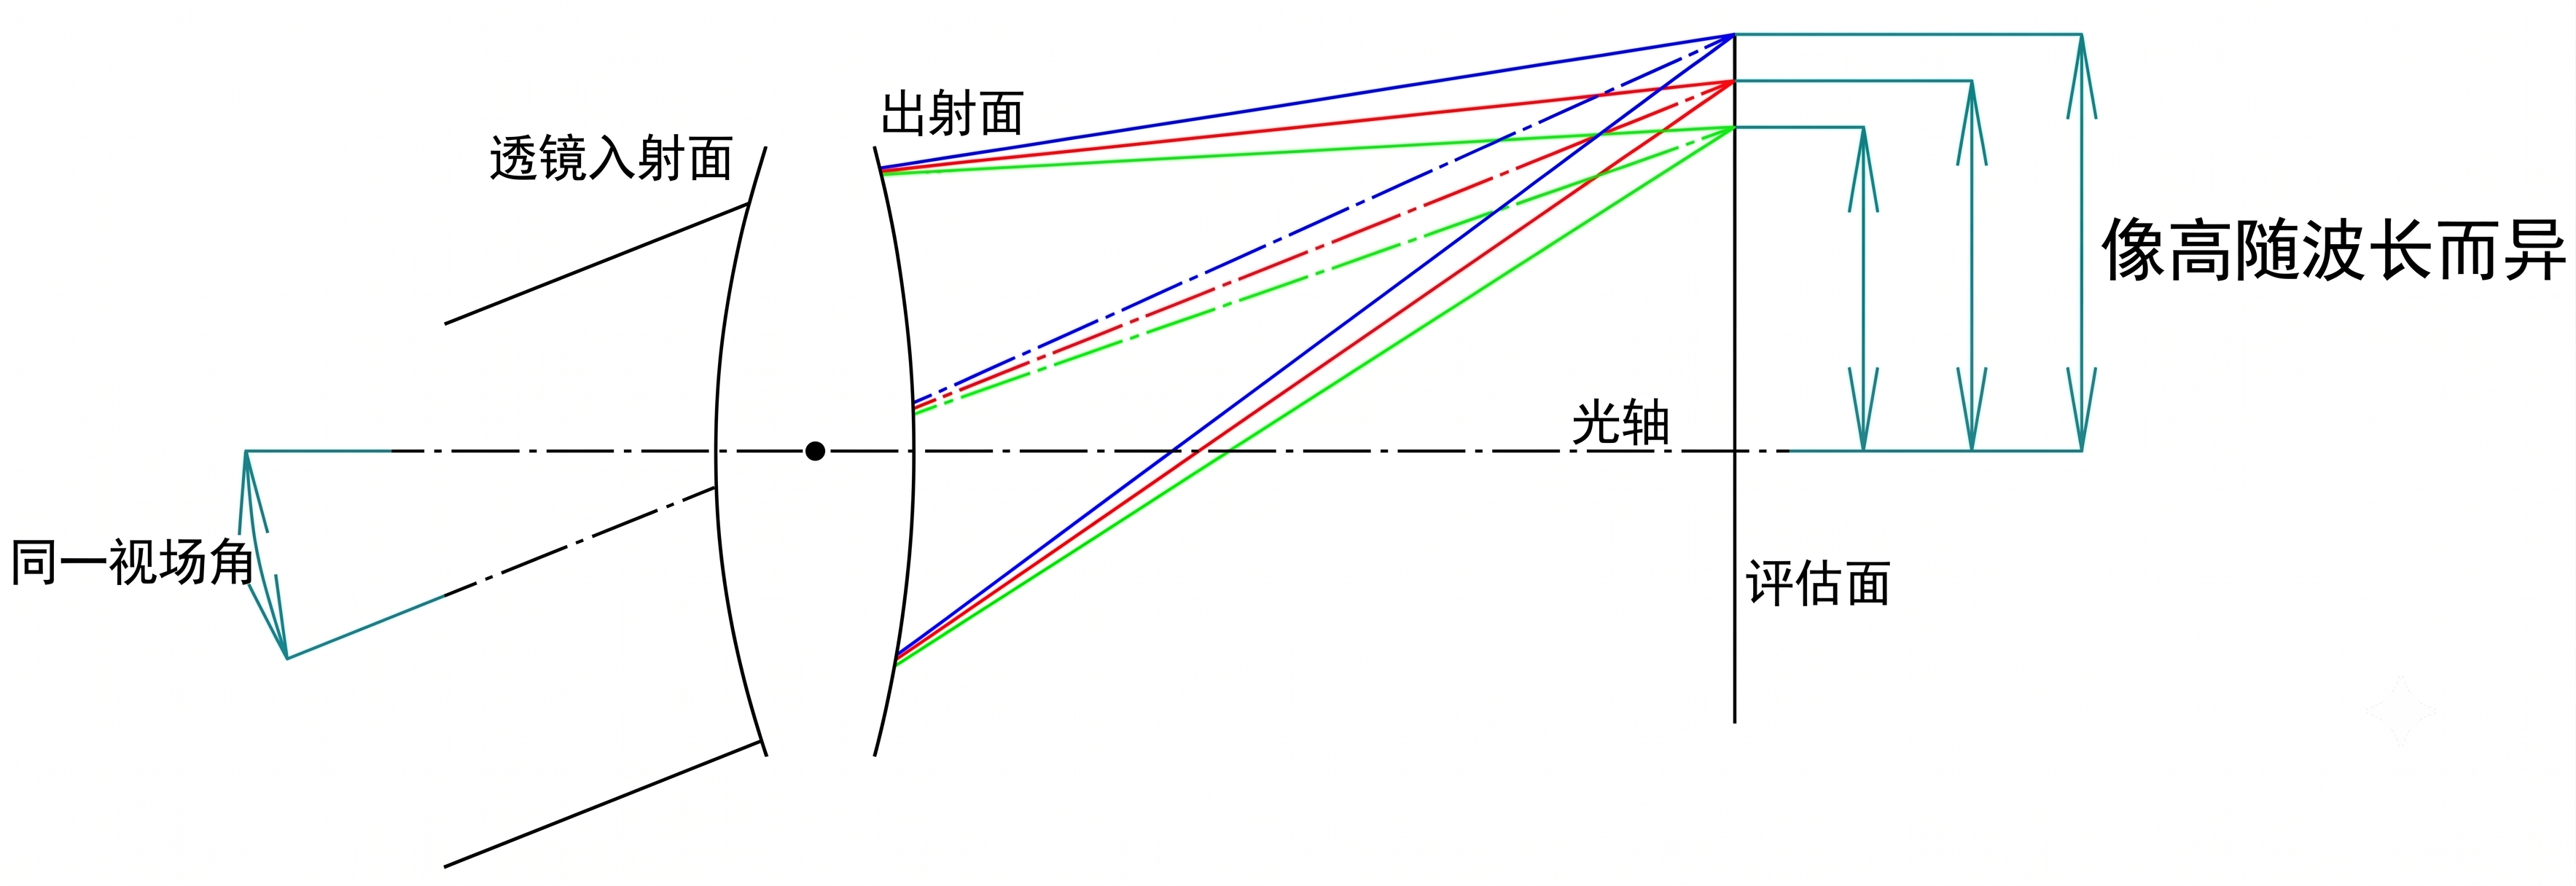
\includegraphics[width=0.98\textwidth]{Figure/图片31.png}\\[3pt]
                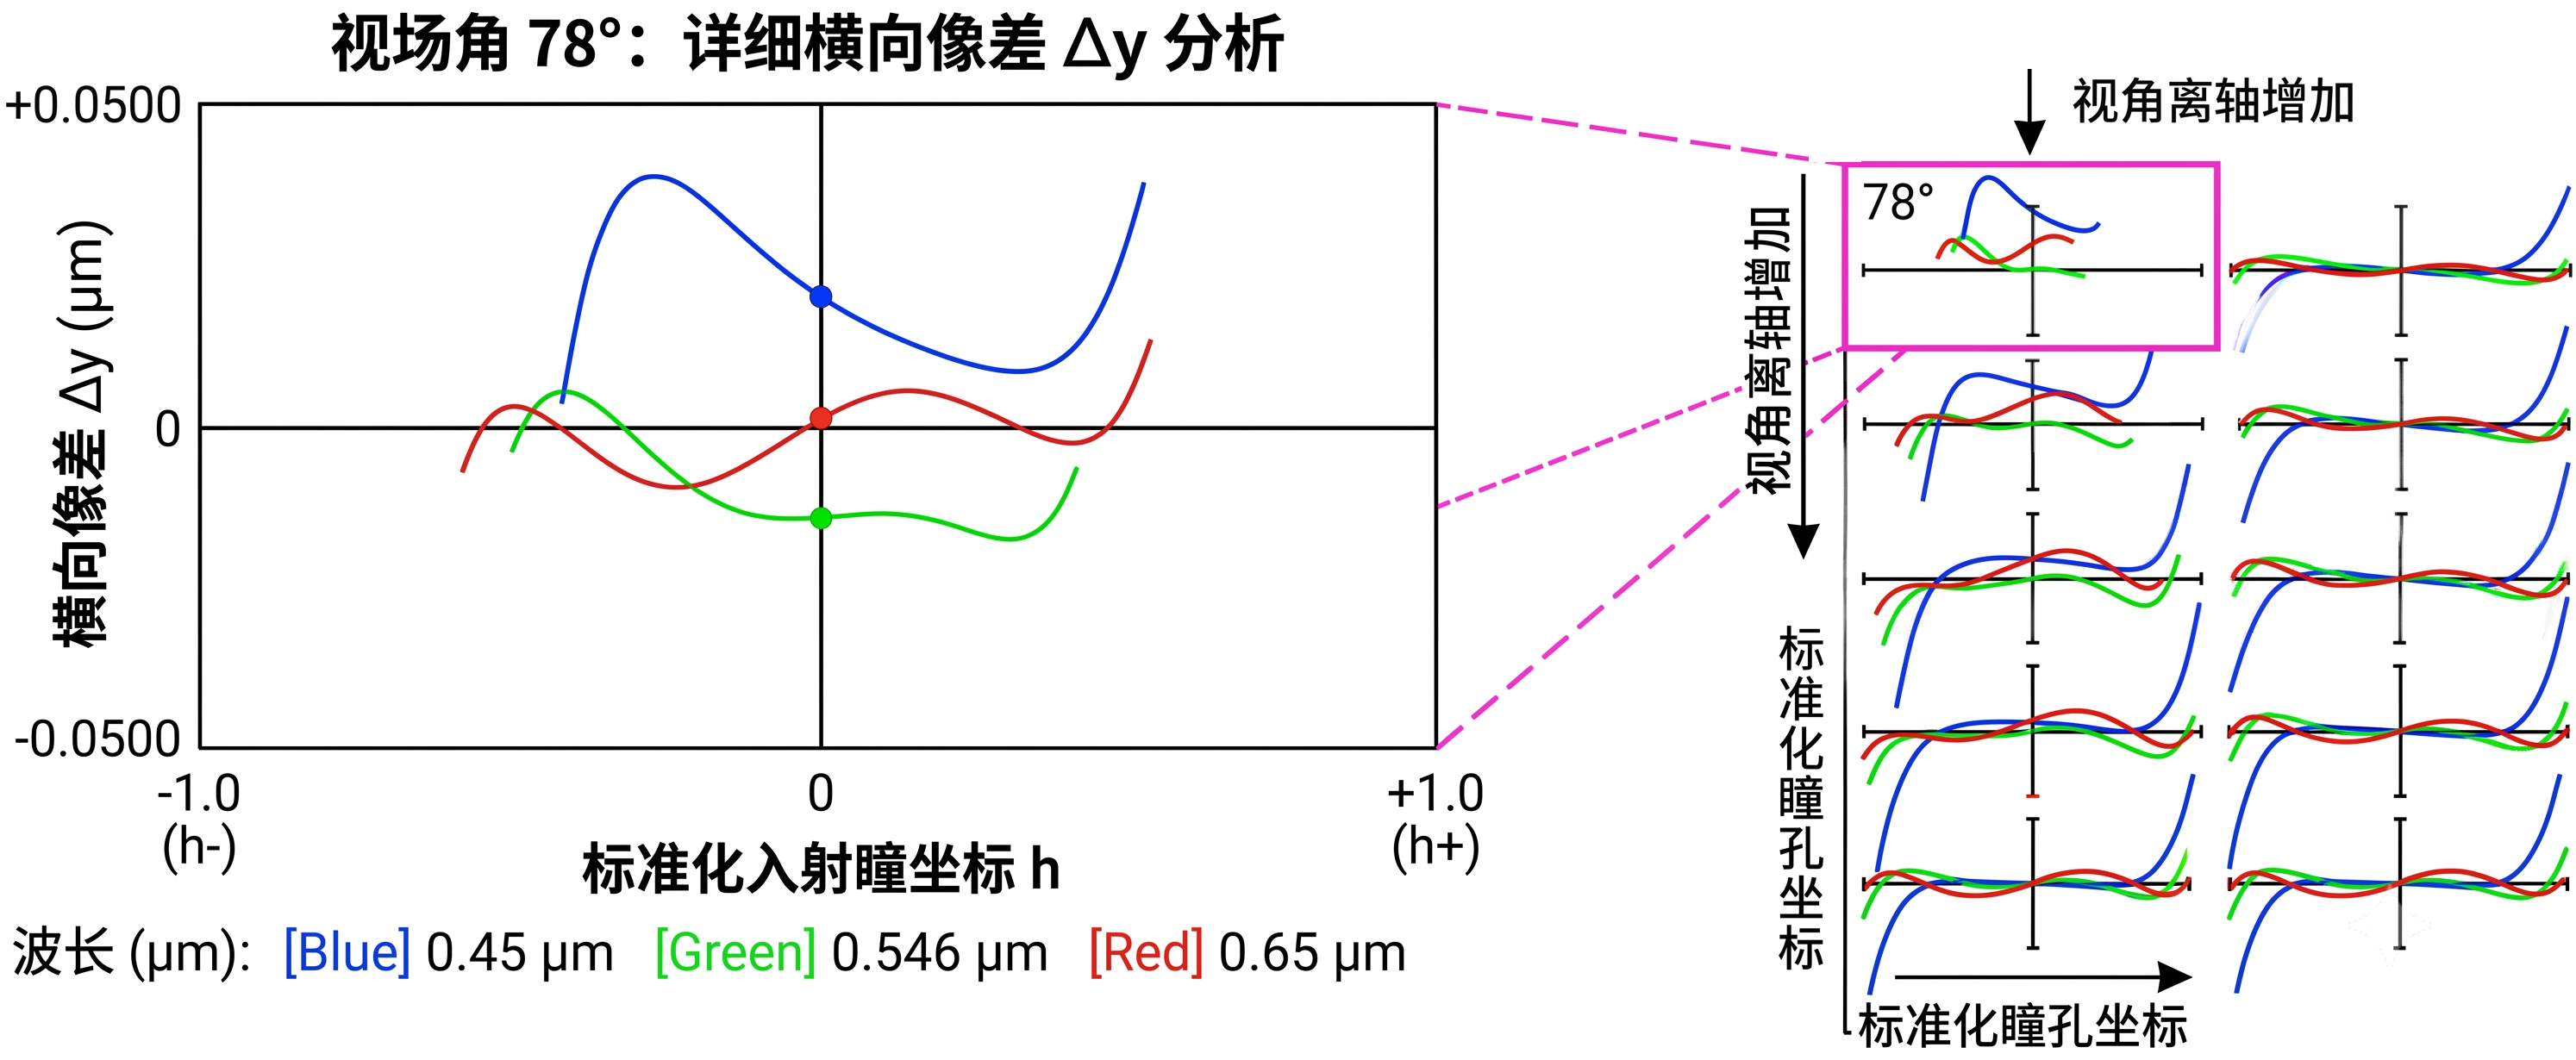
\includegraphics[width=0.98\textwidth]{Figure/图片29.png}
                \caption{倍率色差的光路示意与横向像差图特征}
                \label{fig:lateral_color}
            \end{figure}
        \end{column}
        \hfill
        \begin{column}{.54\textwidth}
            \textbf{倍率色差(横向色差)：}
            \bigbreak
            轴外光束横向像差图与\alert{纵轴交点坐标}因波长不同——不同波长主光线在像面上距光轴\alert{不同高度}成像。

            \bigbreak
            \begin{itemize}
                \item 不同波长以不同倍率成像
                \item 即使轴向色差被完全校正，倍率色差仍可能存在
                \item 在像面\alert{边缘}最为显著
            \end{itemize}

            矫正：\alert{对称光学结构}。
        \end{column}
    \end{columns}
\end{frame}

\englishtitle{Systematic Comparison of Two Chromatic Aberrations}
\begin{frame}{两种色差的系统对比}
    \begin{table}
        \centering
        \small
        \begin{tabular}{p{2.2cm}|p{4.2cm}|p{4.2cm}}
            \toprule
            \textbf{特征} & \textbf{轴向色差} & \textbf{倍率色差} \\
            \midrule
            别名 & 纵色差、位置色差 & 横向色差、放大率色差 \\
            观察位置 & 轴上光束、原点斜率 & 轴外光束、纵轴交点 \\
            像差图表现 & 近轴斜率随波长变化 & 纵轴截距随波长变化 \\
            物理含义 & 焦点位置不同 & 放大率不同 \\
            光束类型 & $0^\circ$ 视场角 & 有视场角 \\
            校正方式 & 消色差双透镜 & 对称光学结构 \\
            \bottomrule
        \end{tabular}
        \caption{轴向色差与倍率色差的全面对比}
        \label{tab:chromatic_compare}
    \end{table}
\end{frame}

\englishtitle{Abbe Number and Dispersion of Optical Glass}
\begin{frame}{阿贝数与光学玻璃的色散特性}
    \begin{columns}[T]
        \begin{column}{.50\textwidth}
            \begin{figure}
                \centering
                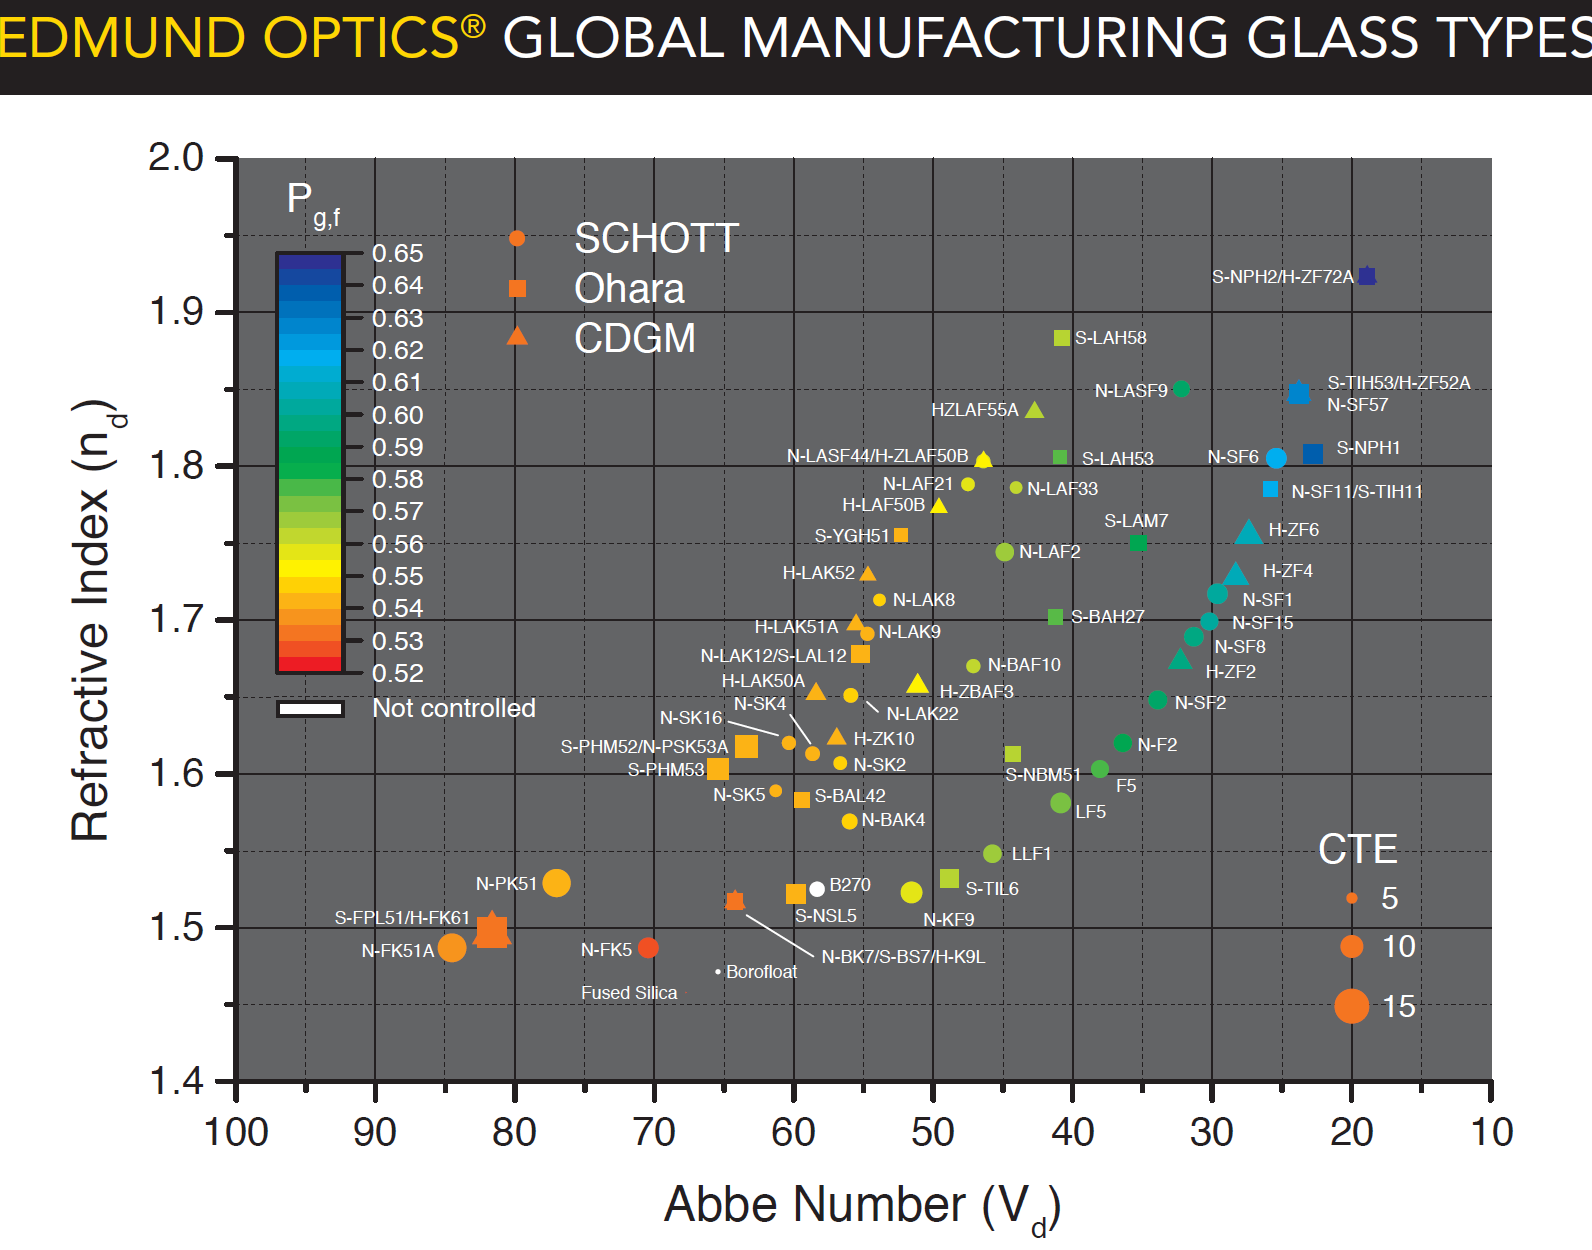
\includegraphics[width=0.95\textwidth]{Figure/Abbe.png}
                \caption{常见光学玻璃的阿贝图——折射率 $n_d$ 与阿贝数 $\nu_d$}
                \label{fig:abbe}
            \end{figure}
        \end{column}
        \hfill
        \begin{column}{.50\textwidth}
            \textbf{阿贝数(Abbe Number)：}
            \begin{equation}
                \nu_d = \frac{n_d - 1}{n_F - n_C}
                \label{eq:abbe}
            \end{equation}
            其中 $n_d$, $n_F$, $n_C$ 分别为 d, F, C 谱线的折射率。

            \bigbreak
            \begin{itemize}
                \item \alert{低阿贝数($\nu_d < 50$)}：高色散(火石玻璃 F 系列)
                \item \alert{高阿贝数($\nu_d > 55$)}：低色散(冕牌玻璃 K 系列)
                \item 消色差设计：搭配高/低阿贝数玻璃，如 BK7+F2
            \end{itemize}
        \end{column}
    \end{columns}
\end{frame}

\englishtitle{Diffraction Limit and Strehl Ratio}
\begin{frame}{衍射极限与斯特列尔比}
    \begin{columns}[T]
        \begin{column}{.60\textwidth}
            \textbf{衍射极限(Diffraction Limit)：}
            即使 $OPD = 0$，受孔径衍射效应限制，点像仍是\alert{艾里斑(Airy Disk)}。

            \bigbreak
            \textbf{斯特列尔比(Strehl Ratio, S.R.)：}
            \begin{equation}
                S.R. \approx \exp\!\left[-\left(\frac{2\pi}{\lambda}\,OPD_{\text{rms}}\right)^2\right]
                \label{eq:strehl}
            \end{equation}

            当像差较小时，可退化为\alert{马瑞夏近似}：
            \begin{equation}
                S.R. \approx 1 - \left(\frac{2\pi}{\lambda}\right)^2 (OPD_{\text{rms}})^2
                \label{eq:marechal}
            \end{equation}
        \end{column}
        \hfill
        \begin{column}{.40\textwidth}
            \begin{block}{瑞利判据}
                当 $|OPD_{\text{PV}}| \le \frac{\lambda}{4}$ 时，
                \alert{$S.R. > 0.8$}，系统达到\alert{衍射极限}。
            \end{block}

            \begin{table}
                \small
                \begin{tabular}{c|c|c}
                    \toprule
                    \textbf{OPD\textsubscript{PV}} & \textbf{S.R.} & \textbf{评价} \\
                    \midrule
                    $<\lambda/4$  & $>0.8$  & 衍射极限 \\
                    $\lambda/4\sim\lambda/2$ & $0.4\sim0.8$ & 可接受 \\
                    $>\lambda/2$ & $<0.4$   & 需矫正 \\
                    \bottomrule
                \end{tabular}
                \caption{像质评估对照}
                \label{tab:strehl_table}
            \end{table}
        \end{column}
    \end{columns}
\end{frame}

\englishtitle{Common Image-Quality Metrics in Optical Design}
\begin{frame}{光学设计中的常用像质评价量}
    \begin{columns}[T]
        \begin{column}{.52\textwidth}
            \begin{block}{几何光学评价}
                \begin{itemize}
                    \item \textbf{横向像差图 / Ray Fan}：最快定位球差、彗差、像散和色差来源
                    \item \textbf{点列图(Spot Diagram)}：观察能量在几何像点附近的扩散范围
                \end{itemize}
            \end{block}

            \begin{block}{波前评价}
                \begin{itemize}
                    \item \textbf{OPD / Wavefront Map}：直接关联瑞利判据和 Strehl 比
                    \item \textbf{PV / RMS}：适合做容差和优化目标的量化指标
                \end{itemize}
            \end{block}
        \end{column}
        \hfill
        \begin{column}{.48\textwidth}
            \begin{block}{频域与能量评价}
                \begin{itemize}
                    \item \textbf{MTF}：回答“某一空间频率还能传多少对比度”
                    \item \textbf{PSF}：回答“点像扩散成什么形状”
                    \item \textbf{圈入能量(Encircled Energy)}：回答“探测器像元内能收进多少能量”
                \end{itemize}
            \end{block}

            \textbf{实用建议：}
            \begin{itemize}
                \item 早期结构选型先看 \alert{Ray Fan + Spot}
                \item 接近完成时重点看 \alert{MTF + RMS OPD + 圈入能量}
                \item 若面向传感器成像，要把\alert{像元尺寸}和截止频率一起考虑
            \end{itemize}
        \end{column}
    \end{columns}
\end{frame}

\subsection{像差分析实战总结}

\englishtitle{Diagnostic Workflow for Transverse Aberration}
\begin{frame}{横向像差图分析流程}
    \begin{block}{系统的像差分析步骤}
        \begin{enumerate}
            \item \textbf{观察轴上光束横向像差图}
            \begin{itemize}
                \item 奇函数曲线 $\rightarrow$ 球差
                \item 原点斜率随波长变化 $\rightarrow$ 轴向色差
            \end{itemize}
            \item \textbf{观察不同视场角的横向像差图}
            \begin{itemize}
                \item 原点斜率变化 $\rightarrow$ 场曲或像散
                \item 子午/弧矢斜率差异 $\rightarrow$ 像散
                \item 横轴宽度变化 $\rightarrow$ 渐晕/光瞳像差
            \end{itemize}
            \item \textbf{检查曲线特征}
            \begin{itemize}
                \item 偶函数对称 $\rightarrow$ 彗差
                \item 上下边缘不对称 $\rightarrow$ 隐性彗差
            \end{itemize}
            \item \textbf{检查波长依赖性}
            \begin{itemize}
                \item 纵轴交点变化 $\rightarrow$ 倍率色差
            \end{itemize}
        \end{enumerate}
    \end{block}
\end{frame}

\englishtitle{Classification and Summary of Aberrations}
\begin{frame}{像差分类总览与横向特征总结}
    \begin{columns}[T,onlytextwidth]
        \begin{column}{.53\textwidth}
            \begin{block}{\footnotesize 表 1\quad 光学系统像差的完整分类}
                \centering
                \scriptsize
                \setlength{\tabcolsep}{2.2pt}
                \renewcommand{\arraystretch}{1.16}
                \resizebox{\linewidth}{!}{%
                    \begin{tabular}{ccccc}
                        \toprule
                        \multicolumn{2}{c}{\textbf{物点位置}} & \textbf{像差类型} & \textbf{影响因素} & \textbf{高斯像面上的像} \\
                        \midrule
                        \multirow{3}{*}{轴上物点}
                        & 单色                & 球差          & 孔径                   & 单色弥散圆斑 \\
                        \cmidrule(lr){2-5}
                        & \multirow{2}{*}{复色}
                                              & 色球差        & 孔径、波长              & \multirow{2}{*}{彩色弥散圆斑} \\
                        &                     & 位置(轴向)色差 & 波长                  & \\
                        \midrule
                        \multirow{5}{*}{轴外物点}
                        & \multirow{4}{*}{单色}
                                              & 彗差(正弦差)  & 孔径、视场              & \multirow{5}{*}{复杂弥散斑} \\
                        &                     & 细光束像散     & 视场                  & \\
                        &                     & 场曲          & \multirow{2}{*}{大物面} & \\
                        &                     & 畸变          &                      & \\
                        \cmidrule(lr){2-5}
                        & 复色                & 倍率色差       & 波长                  & \\
                        \bottomrule
                    \end{tabular}%
                }
                \label{tab:aberration_classification}
            \end{block}
        \end{column}
        \hfill
        \begin{column}{.45\textwidth}
            \begin{block}{\footnotesize 表 2\quad 横向像差图特征总结}
                \centering
                \scriptsize
                \setlength{\tabcolsep}{2.4pt}
                \renewcommand{\arraystretch}{1.85}
                \resizebox{\linewidth}{!}{%
                    \begin{tabular}{cccc}
                        \toprule
                        \textbf{像差类型} & \textbf{曲线特征} & \textbf{函数类型} & \textbf{离焦改善} \\
                        \midrule
                        离焦     & 通过原点的直线       & 奇函数，$h^1$ & \alert{可完全校正} \\
                        球差     & 三次曲线             & 奇函数，$h^3$ & 部分改善 \\
                        彗差     & 二次曲线             & 偶函数，$h^2$ & \alert{否} \\
                        场曲     & 原点附近斜率变化     & 奇函数，$h^1$ & 部分改善 \\
                        像散     & 子午/弧矢斜率不同    & --            & 部分改善 \\
                        轴向色差 & 原点斜率随波长变化   & --            & 需消色差设计 \\
                        倍率色差 & 纵轴交点随波长变化   & --            & 需对称结构 \\
                        \bottomrule
                    \end{tabular}%
                }
                \vspace{8pt}
                \label{tab:aberration_summary}
            \end{block}
        \end{column}
    \end{columns}

    \vspace{4pt}
    {\footnotesize \alert{两大类：}单色像差(球差/彗差/像散/场曲/畸变)影响成像清晰度和物像相似度；色差(位置色差/倍率色差)源于 $n(\lambda)$ 导致的色散。}
\end{frame}

\englishtitle{Key Takeaways of Aberration Analysis}
\begin{frame}{像差分析的核心要点}
    \begin{itemize}
        \item 横向像差图中包含\alert{离焦、球差、彗差、场曲、像散、色差}的复合信息
        \item 分析的关键在于\alert{分解各分量}，而非整体判断
        \item 原点附近(近轴区域)：场曲、像散、色差占主导
        \item 边缘光线区域：球差和彗差显著体现
        \item 画角依赖性和波长依赖性是区分色差的关键
        \item 子午/弧矢分量的对比是识别像散的唯一方法
        \item 镜头设计没有捷径——但掌握了横向像差图的解读，就能"聆听镜头参数发出的像差之声"
    \end{itemize}
\end{frame}
